\documentclass[dissertation.tex]{subfiles}
\begin{document}

This appendix contains figures that visualize the Kernel Density Estimation
(KDE) discrepancies when using activation function $\tanh$ and ReLu.
\begin{itemize}
  \item{
      $\tanh$ - see \autoref{figKDETS}, \autoref{figNetworkShapes}: Almost every
      figure that visualizes a NN with the $\tanh$ activation function has a
      pronounced dip in label information, this observation seems to exists
      regardless of network shape or training size
    }
  \item{
      ReLu - see \autoref{figKDETSRelu}, \autoref{figNetworkShapesReLu}: Only
      some of the ReLu NNs experience the same dip in information in the second
      layer.
    }
\end{itemize}
I was not able to find the source of this error. In the paper by Saxe their
method does not seem to suffer from the same issue. In order to not introduce
potentially wrong data into the project I decided to leave out information
planes that were measured with the KDE MIE.

In order to implement the KDE MIE I used the same code that was used by Saxe in
his paper.

% KDE Training Set
\begin{figure}[ht]
  \centering
  \begin{subfigure}[t]{0.32\textwidth}
    \centering
    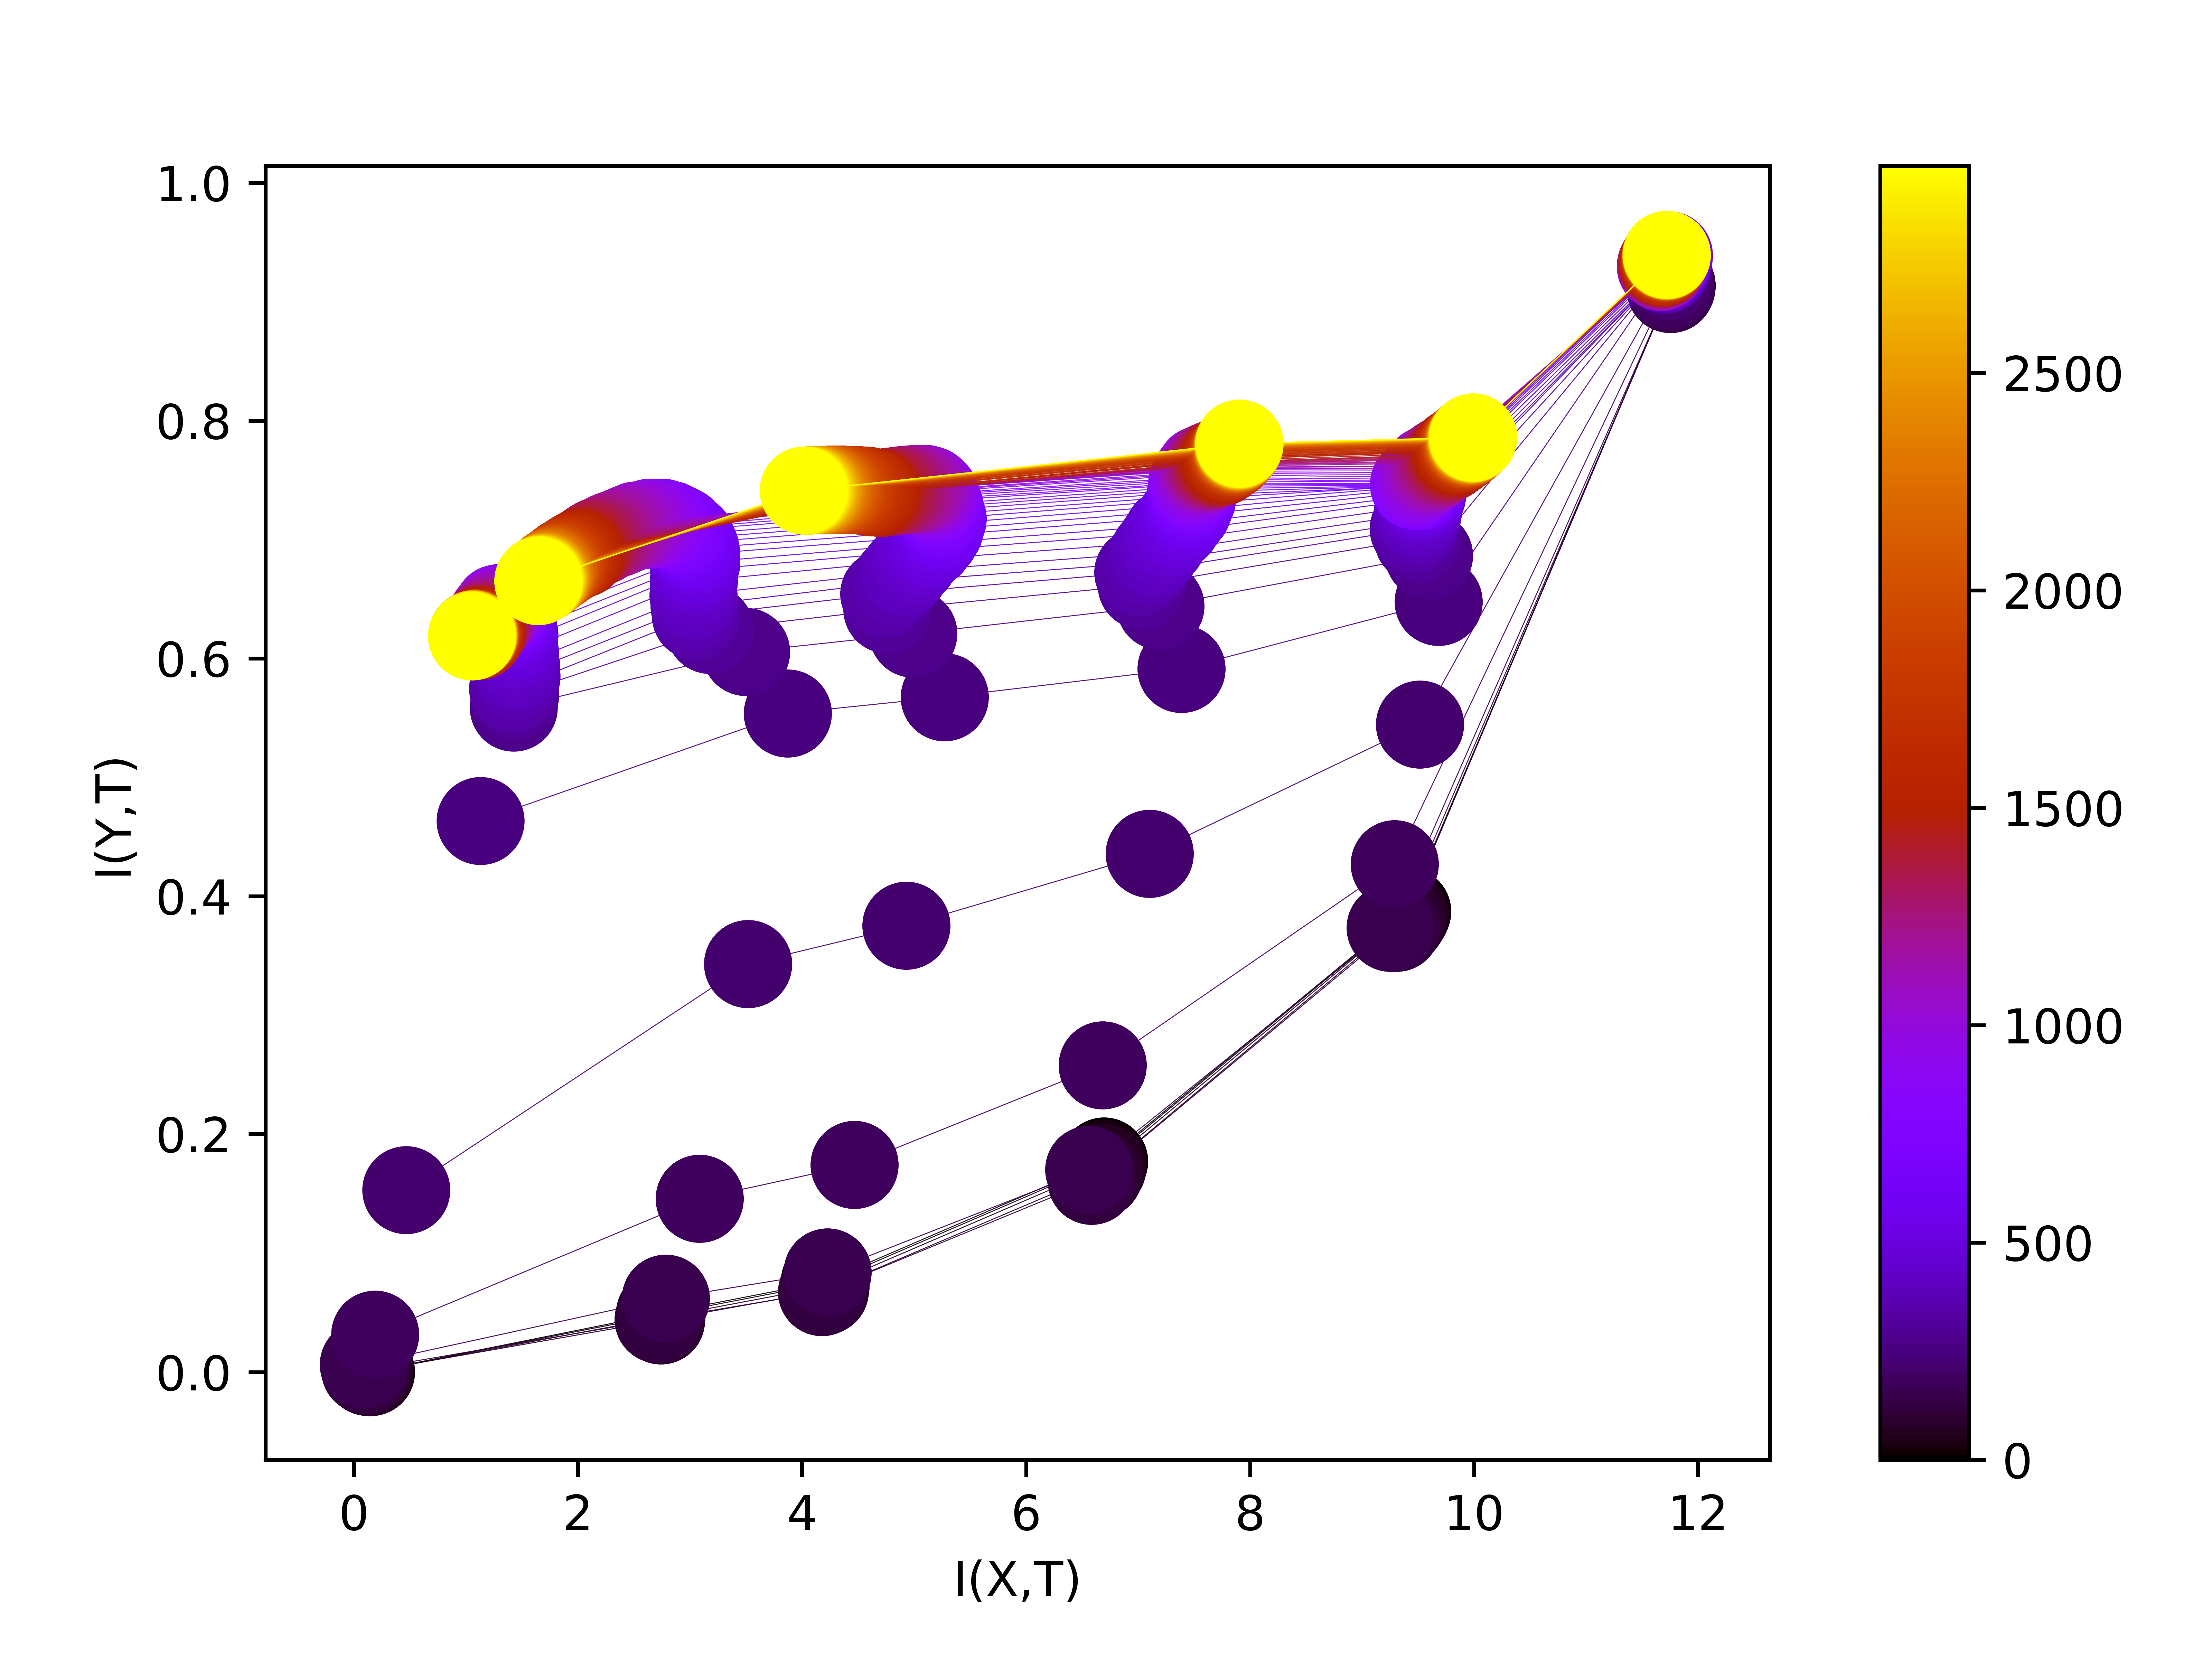
\includegraphics[width=\textwidth]{figs/eval/trainingSize/KDE20.png}
    \caption{
      Training size - 20\%
    }
    \label{figKDETS20}
  \end{subfigure}
  \begin{subfigure}[t]{0.32\textwidth}
    \centering
    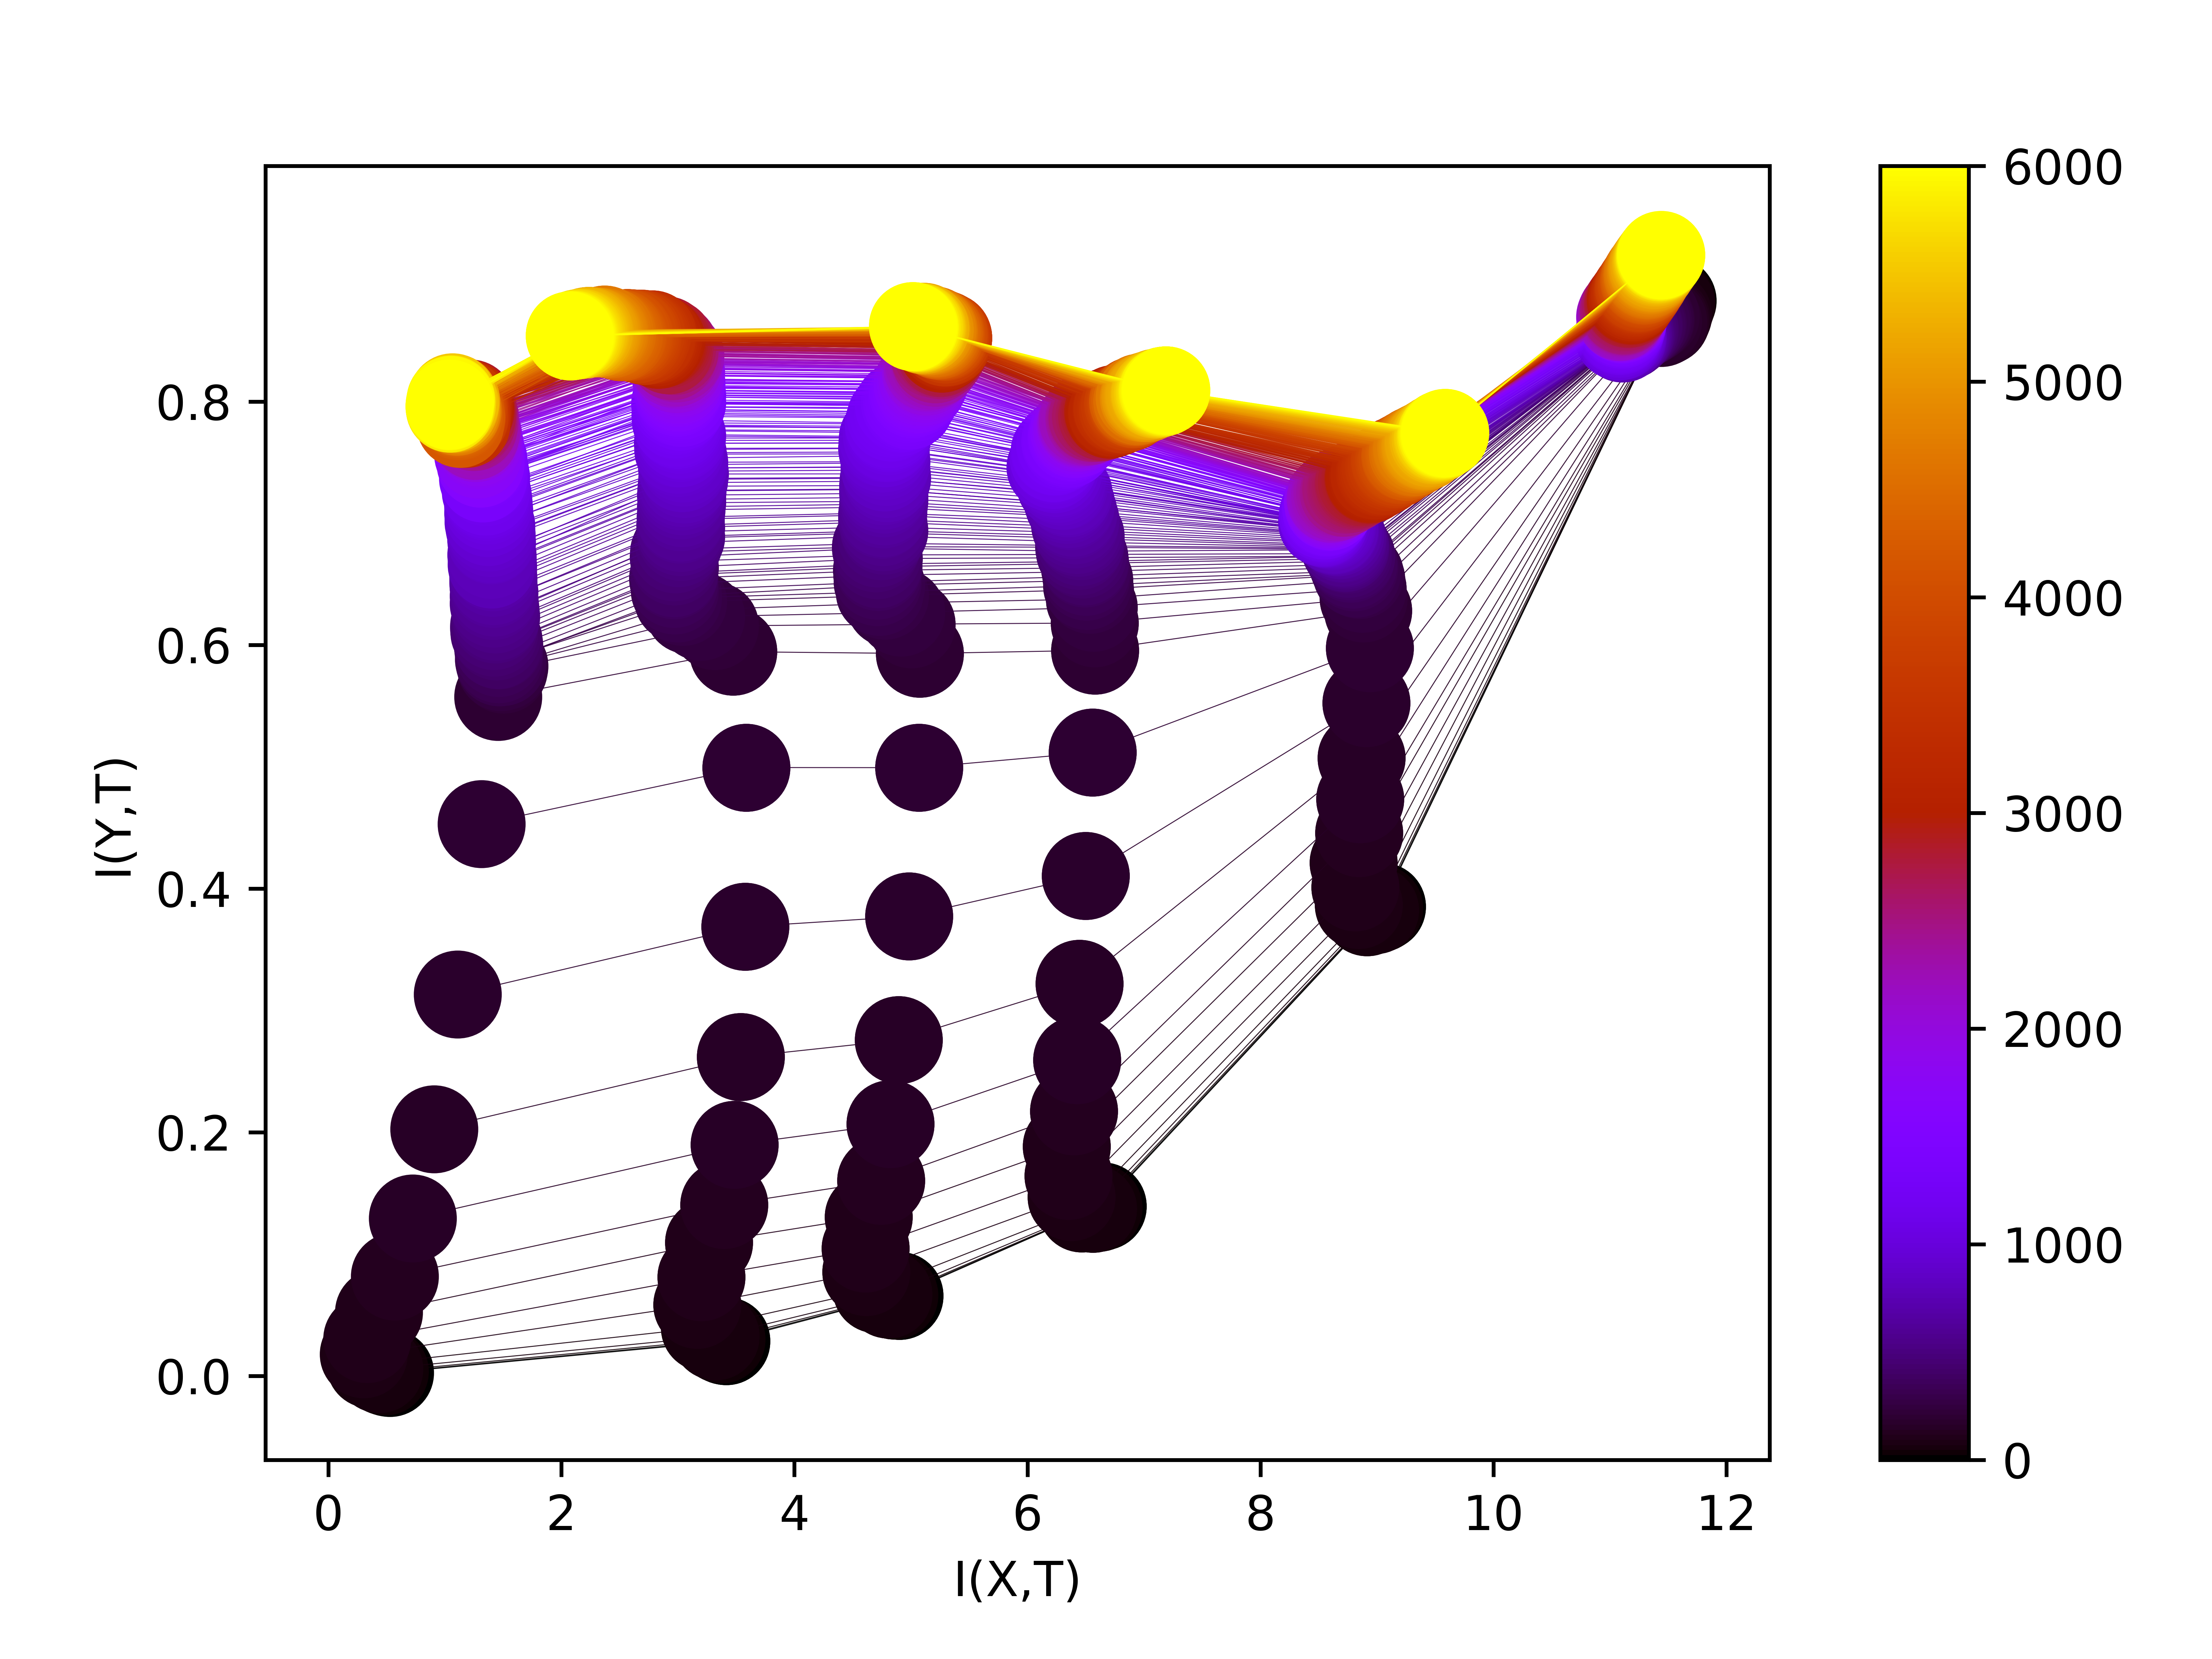
\includegraphics[width=\textwidth]{figs/eval/trainingSize/KDE40.png}
    \caption{
      Training size - 40\%
    }
    \label{figKDETS40}
  \end{subfigure}
  \begin{subfigure}[t]{0.32\textwidth}
    \centering
    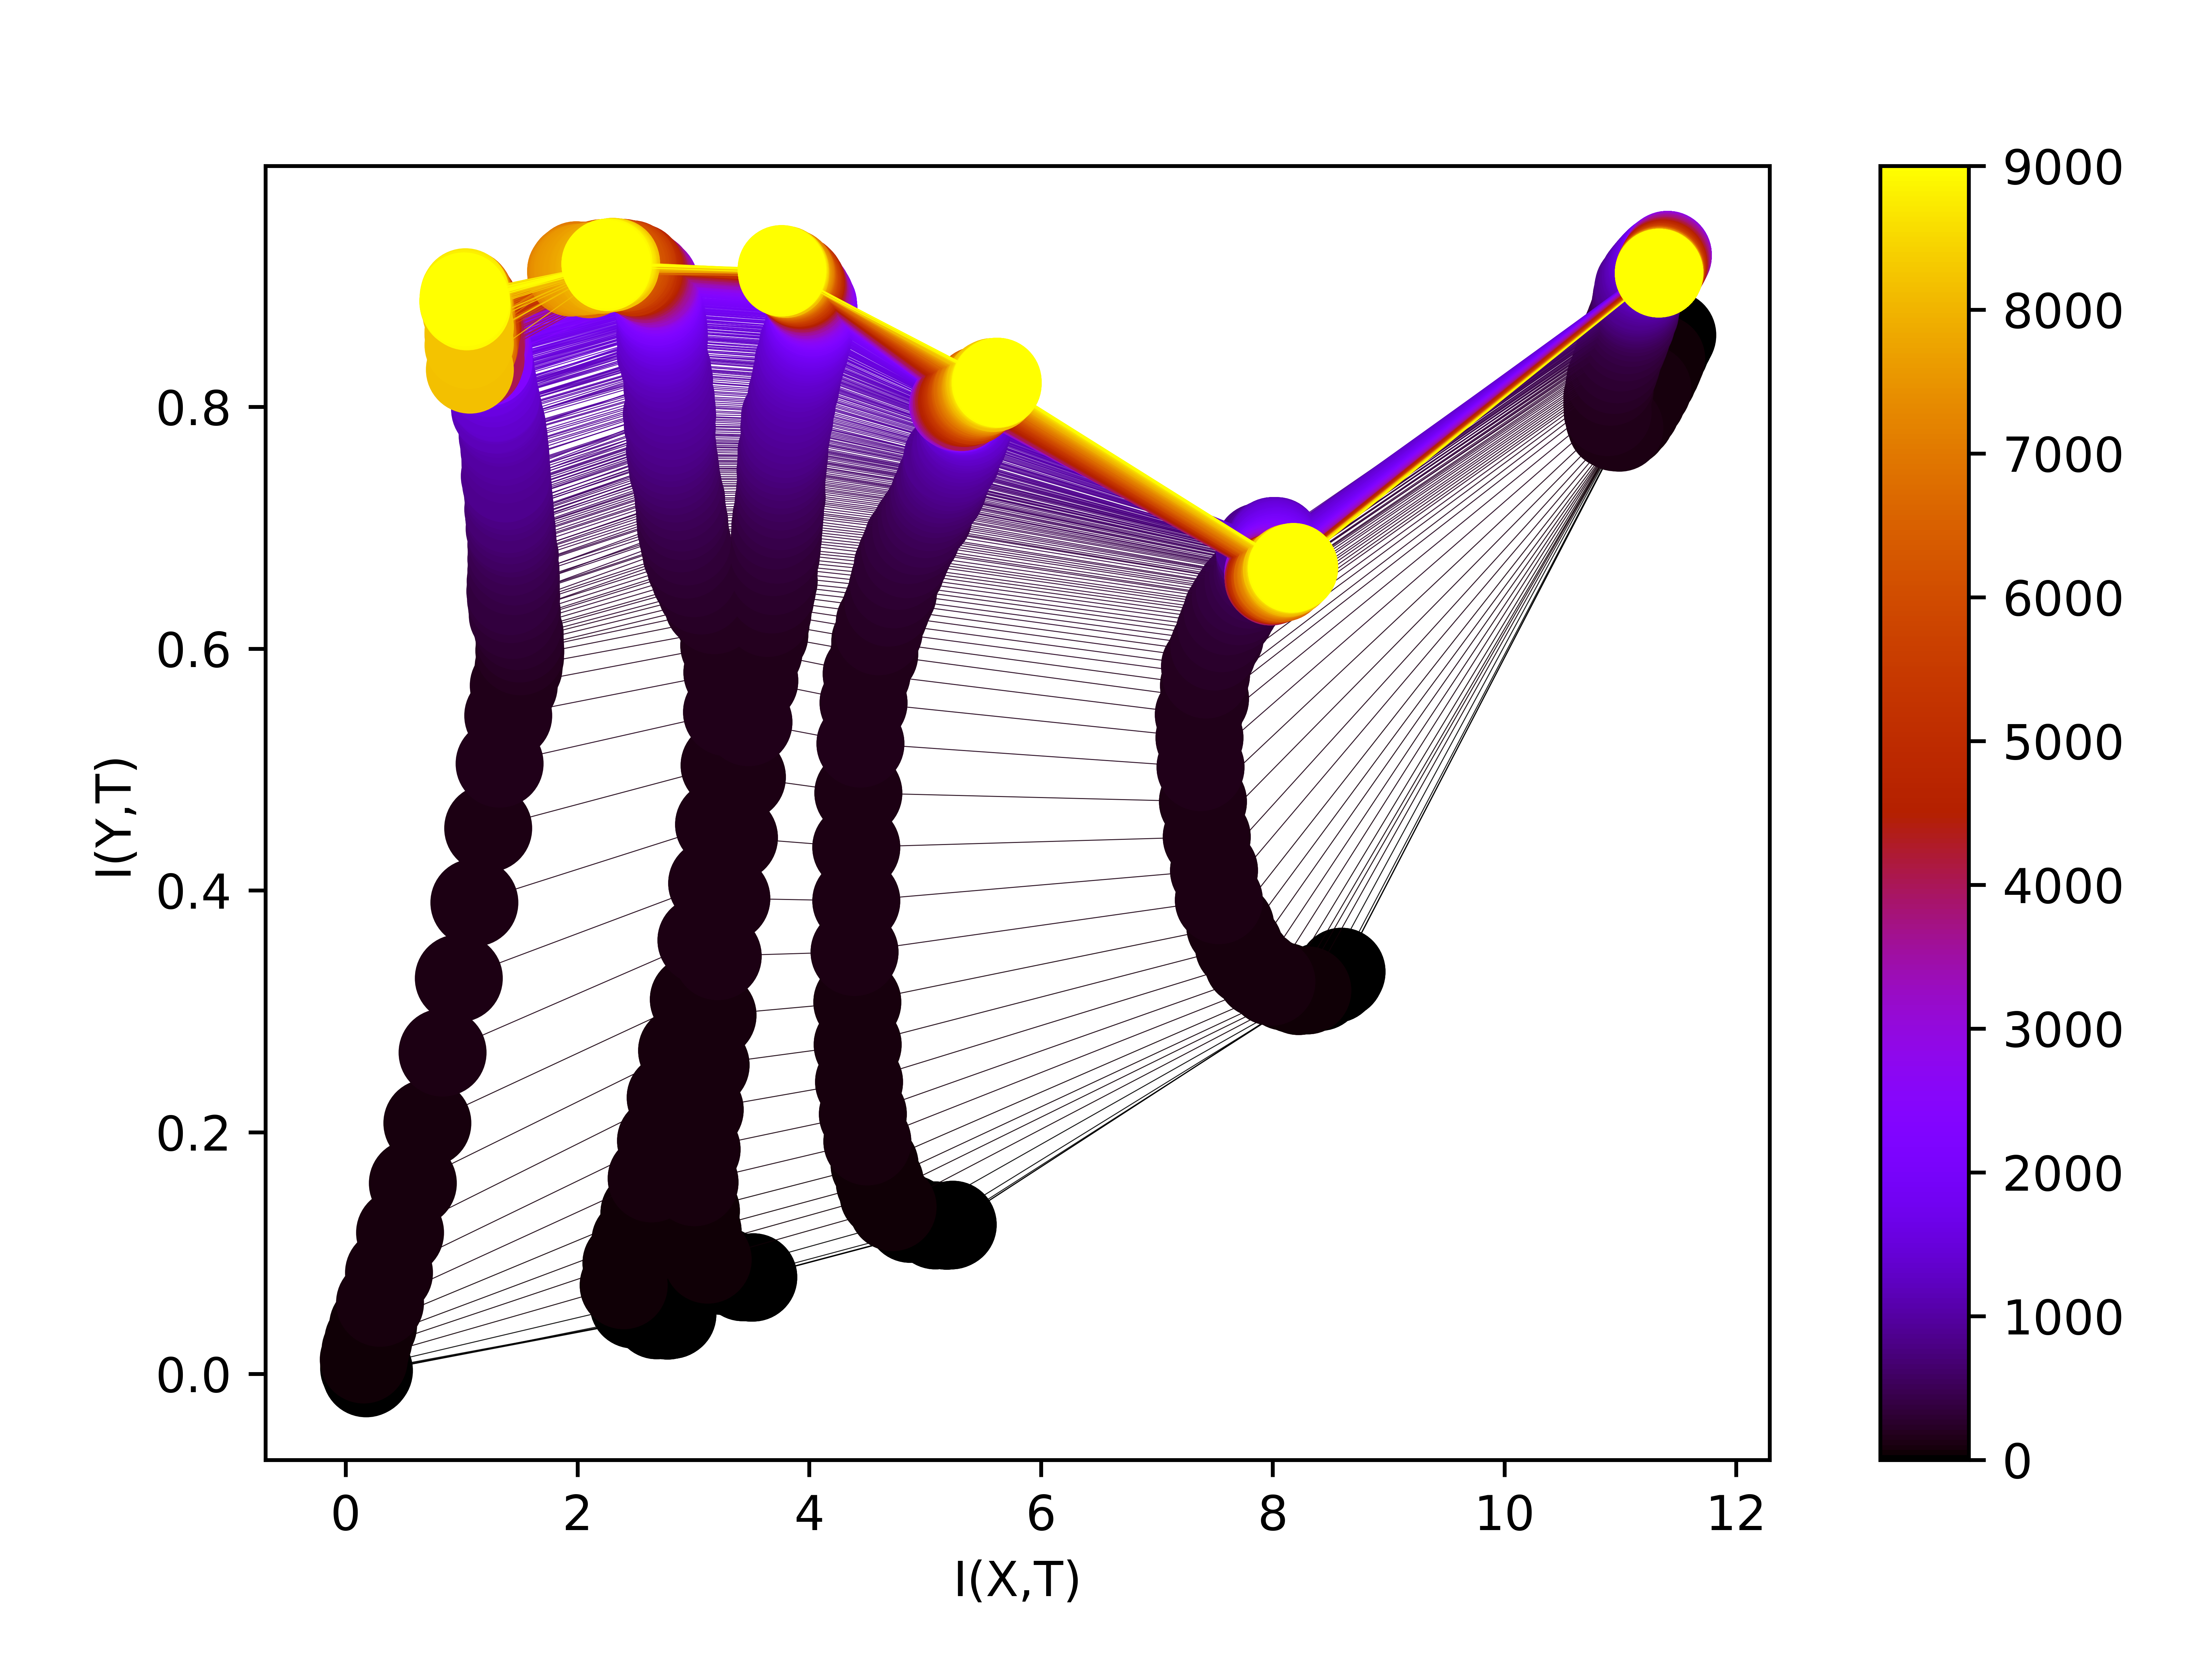
\includegraphics[width=\textwidth]{figs/eval/trainingSize/KDE70.png}
    \caption{
      Training size - 70\%
    }
    \label{figKDETS70}
  \end{subfigure}
  \caption{
      $\tanh$: Demonstrating KDE for different training sizes.  Tweaking training
      size for Tishby's KDE MIE. Hyperparameters: Dataset - Tishby's, activation
      function - $\tanh$, batch size - 512, network shape 12,10,8,6,4,2.
    }
  \label{figKDETS}
\end{figure}

\begin{figure}[ht]
  \centering
  \begin{subfigure}[t]{0.32\textwidth}
    \centering
    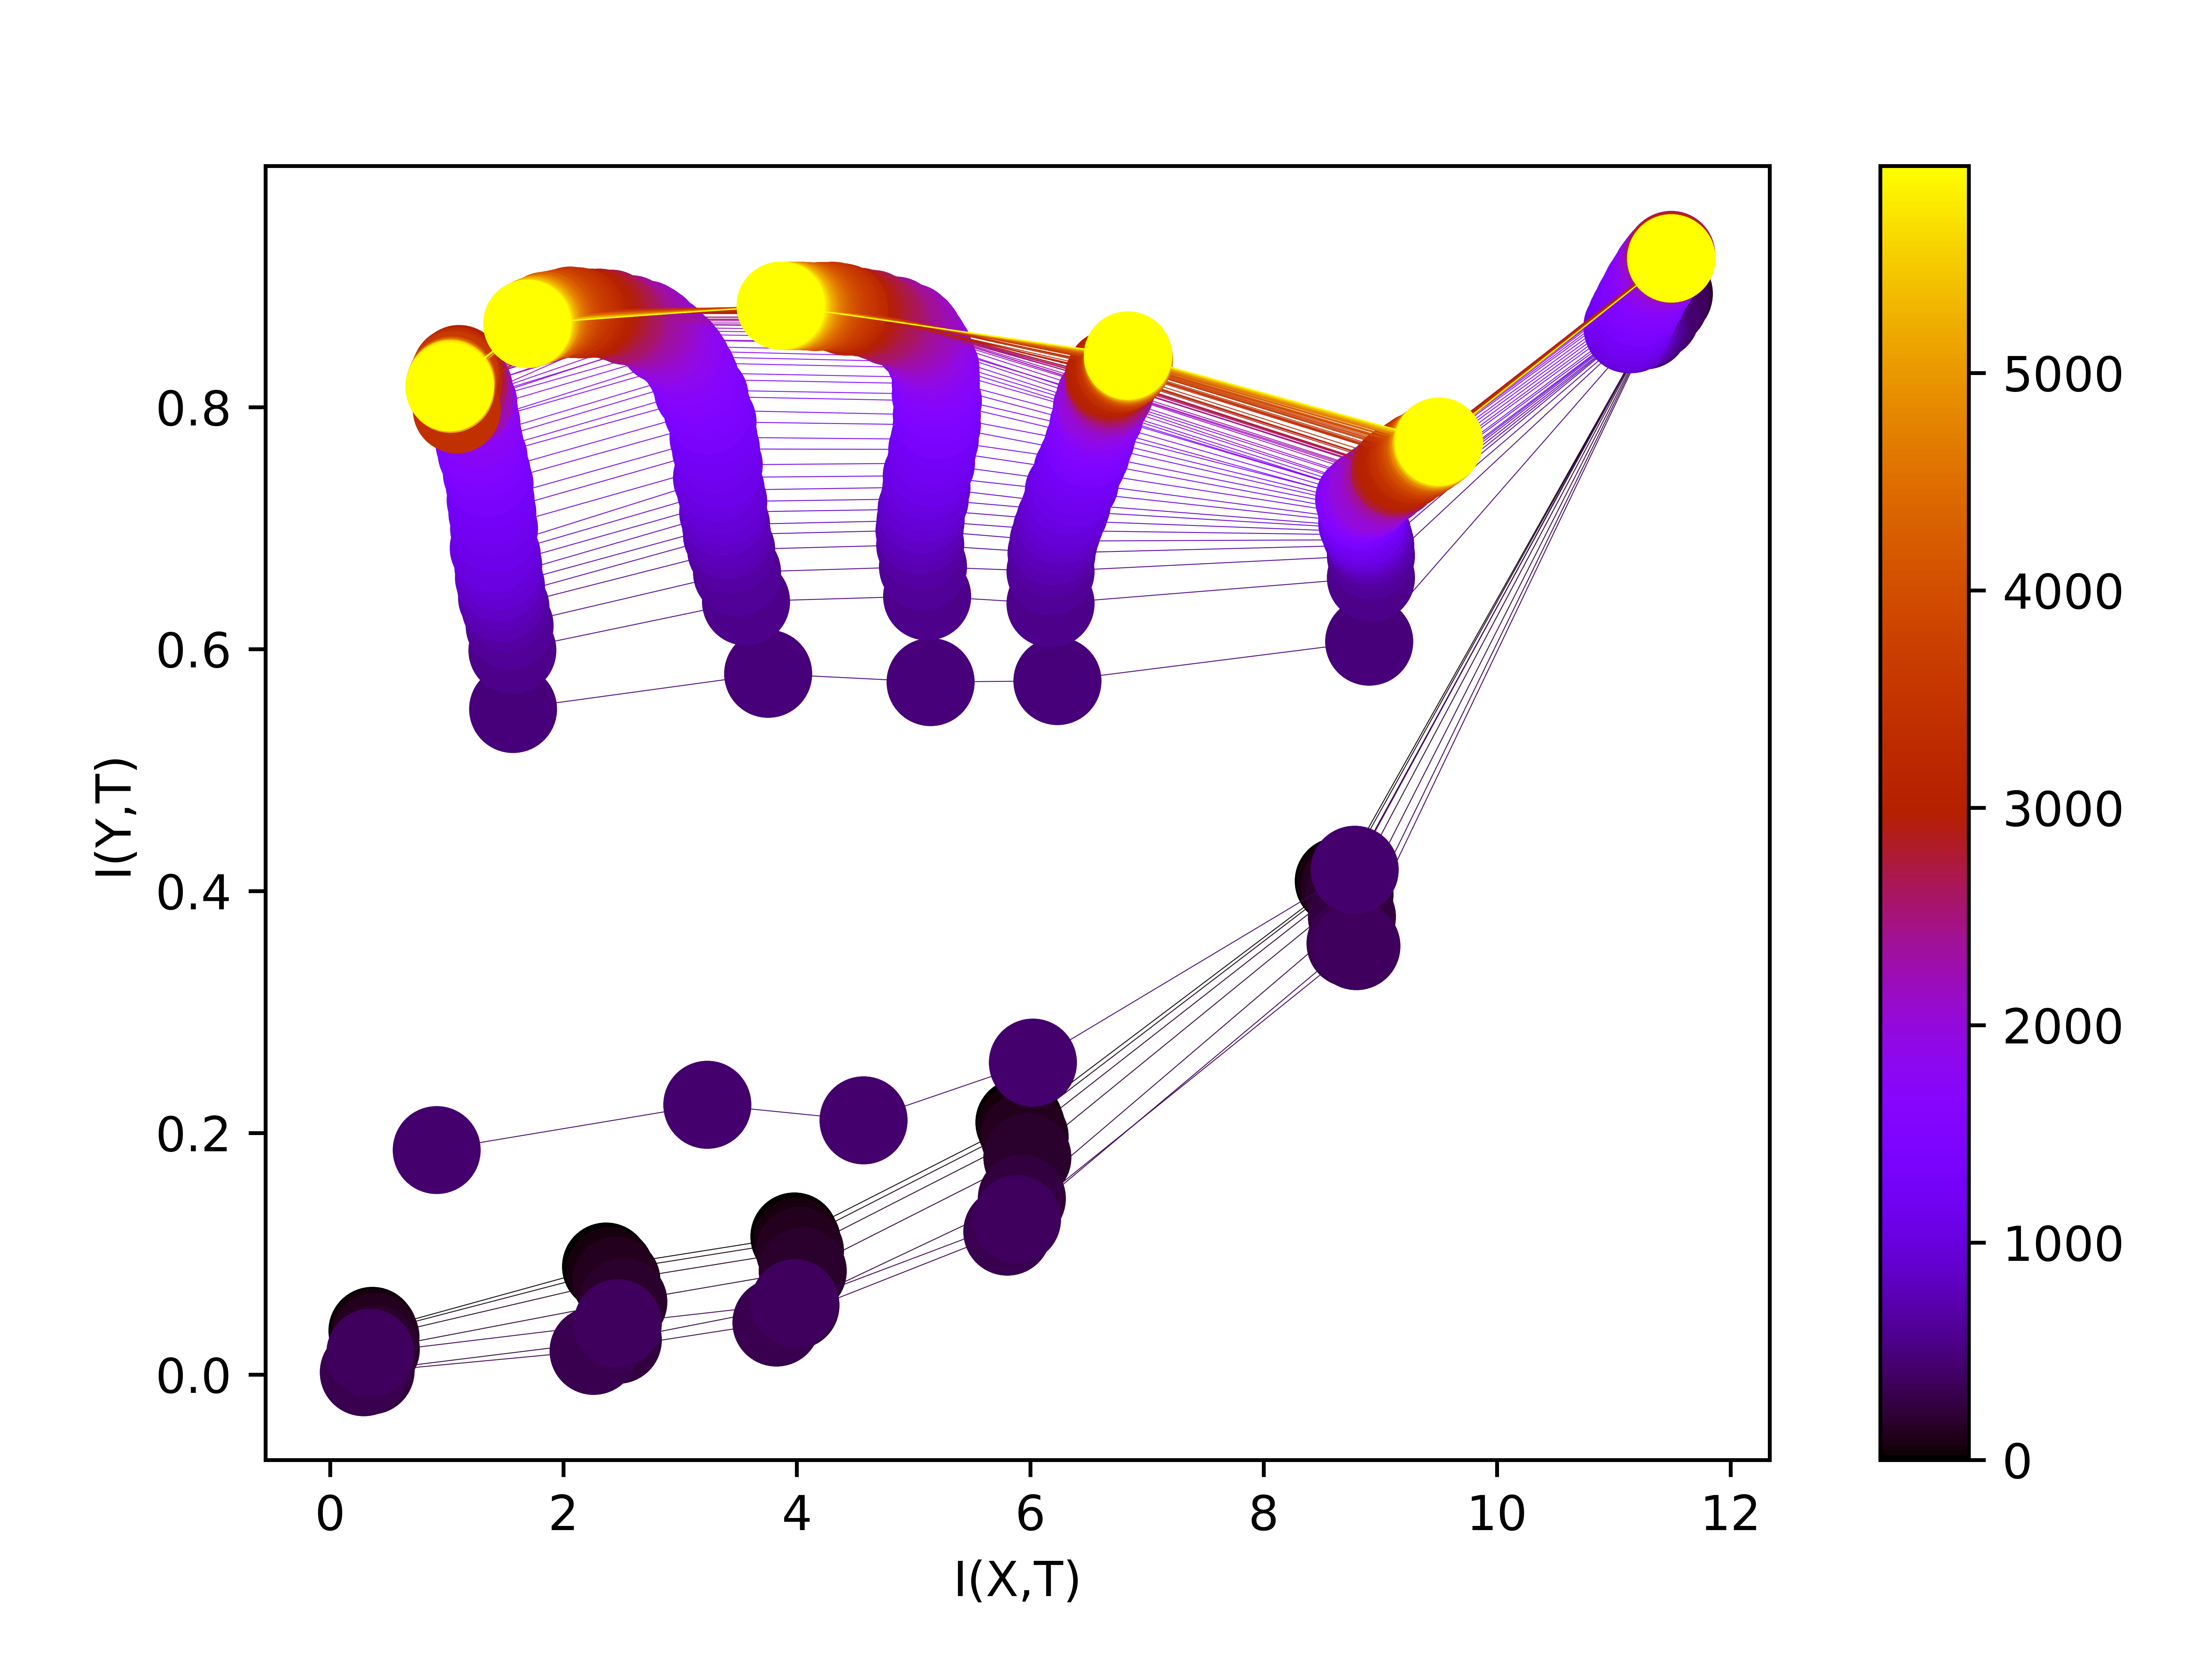
\includegraphics[width=\textwidth]{figs/eval/networkShape/KDE10,8,6,4.png}
    \caption{
      Network Shape - 12,10,8,6,4,2, Default
    }
    \label{figNetworkShape2}
  \end{subfigure}
  \hfill
  \begin{subfigure}[t]{0.32\textwidth}
    \centering
    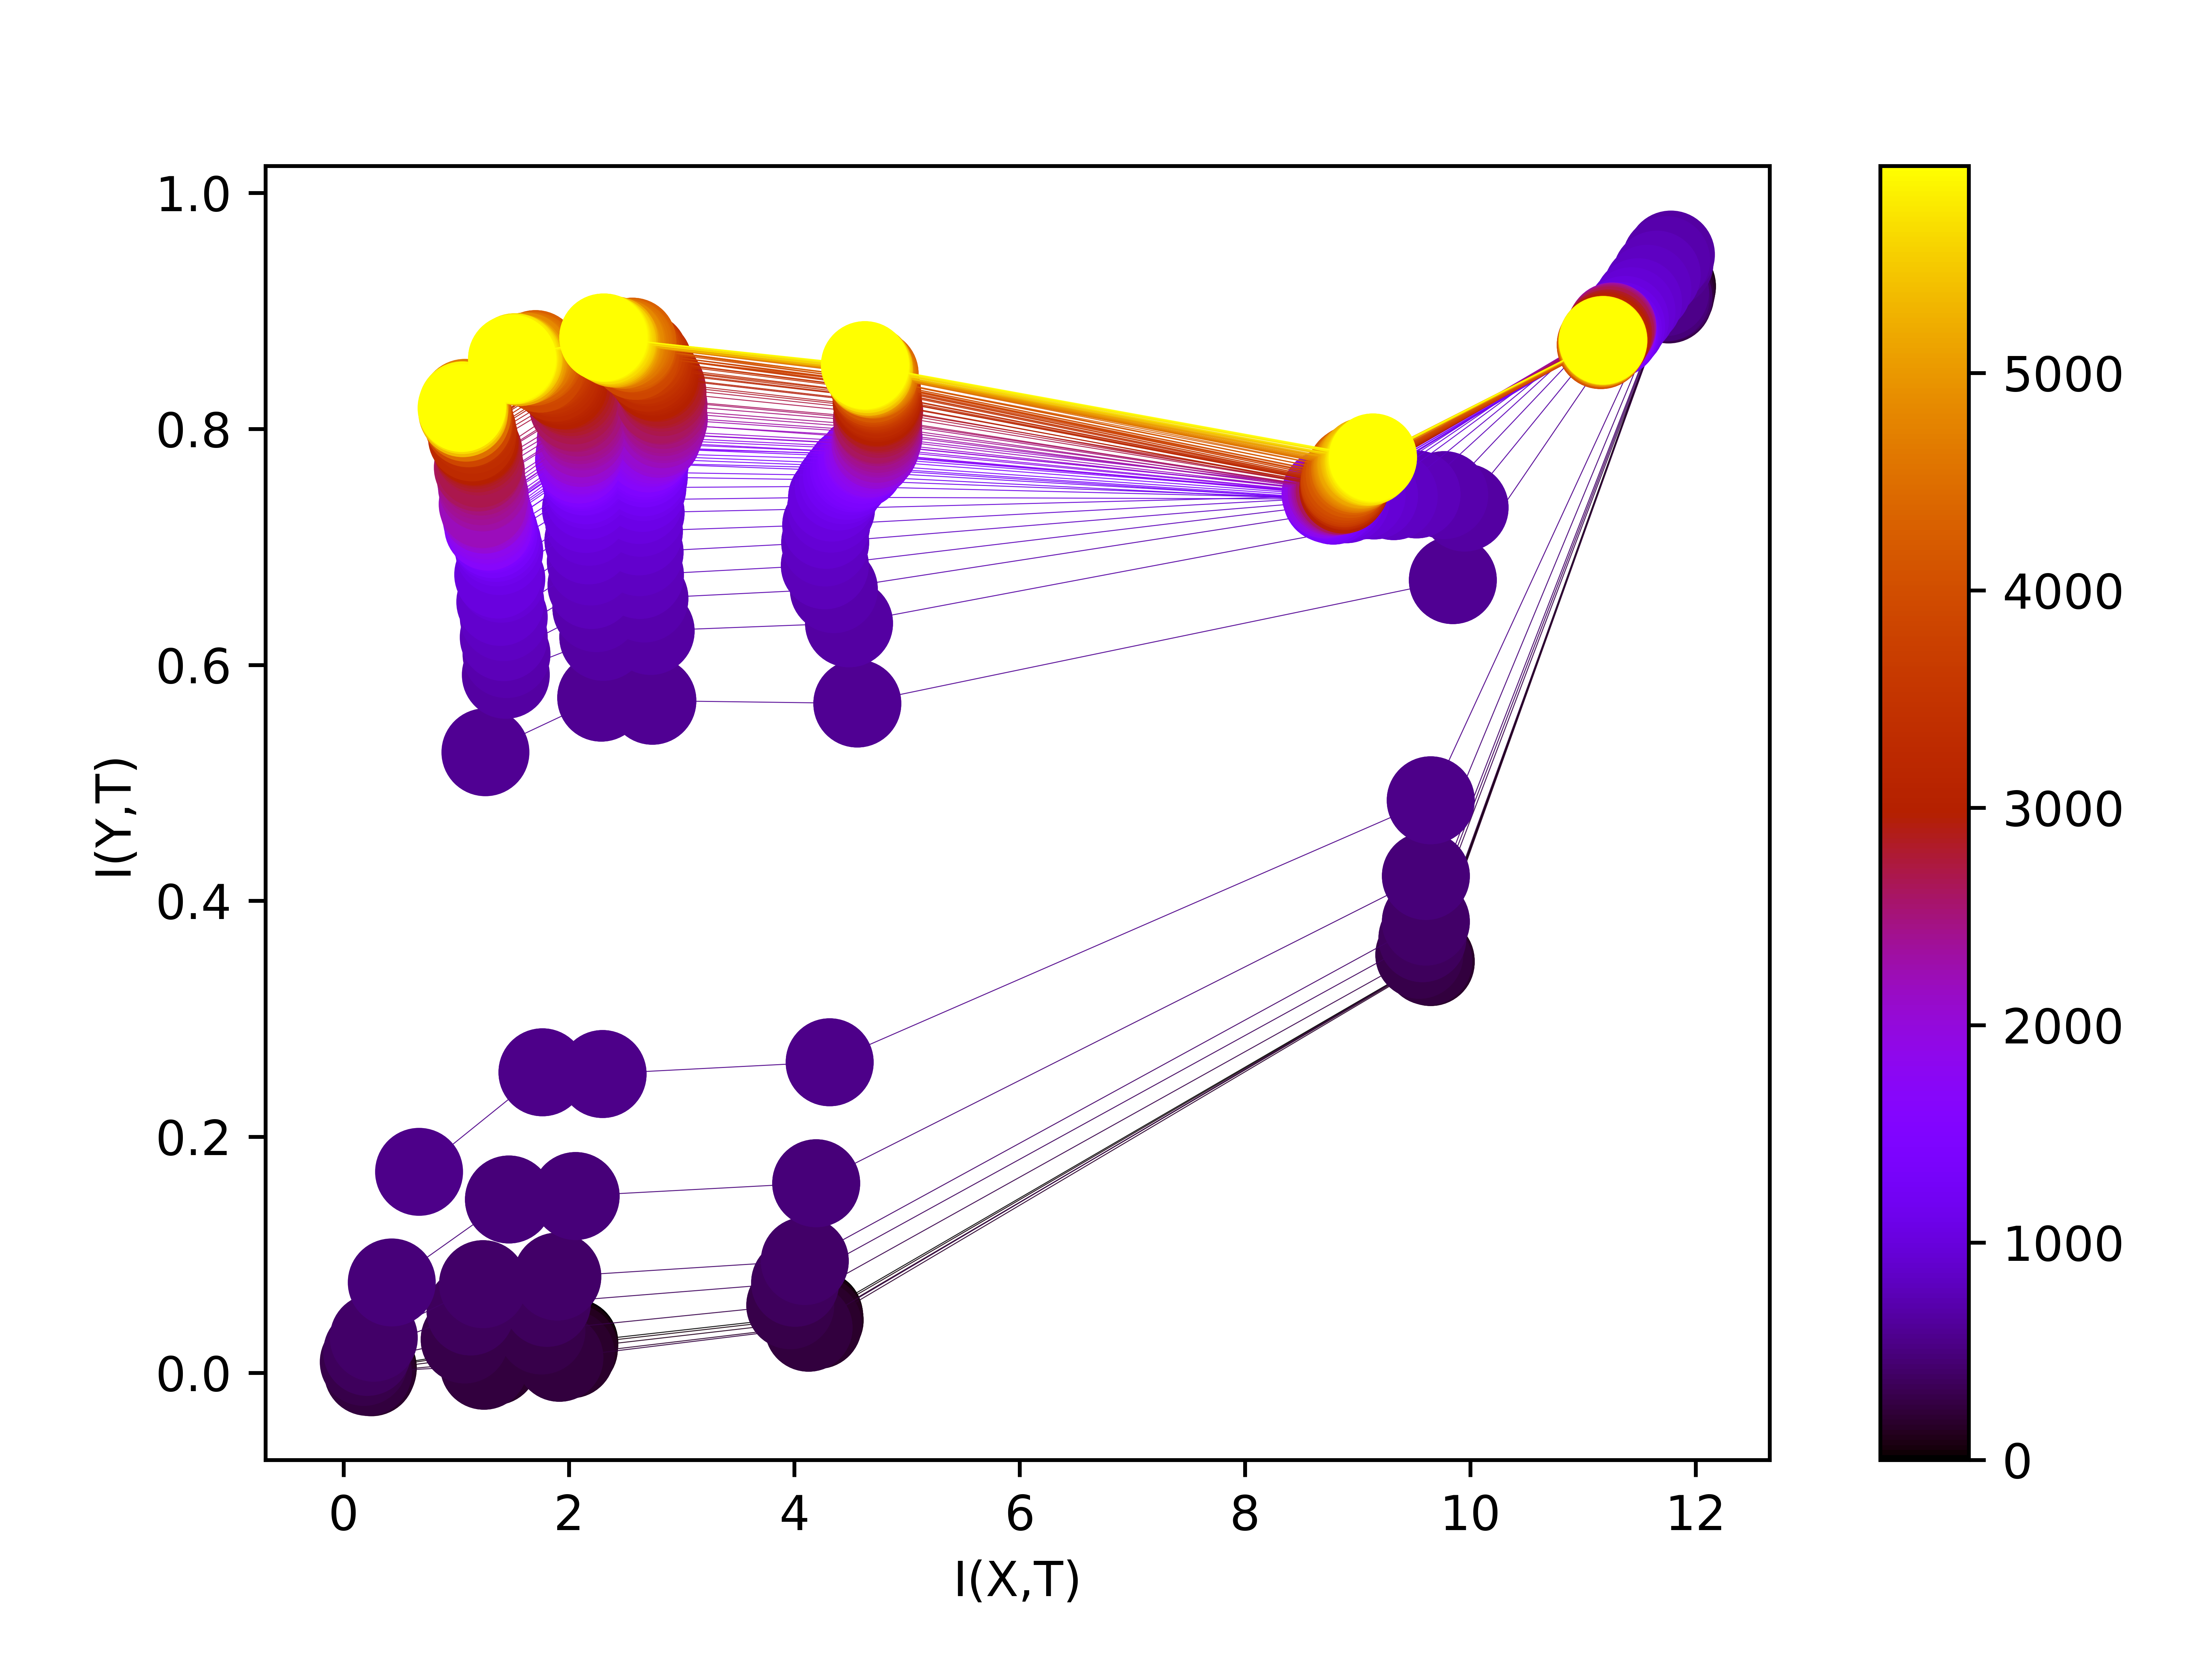
\includegraphics[width=\textwidth]{figs/eval/networkShape/KDE10,4,2,2.png}
    \caption{
      Network Shape - 12,10,4,2,2,2
    }
    \label{figNetworkShapeDefault}
  \end{subfigure}
  \hfill
  \begin{subfigure}[t]{0.32\textwidth}
    \centering
    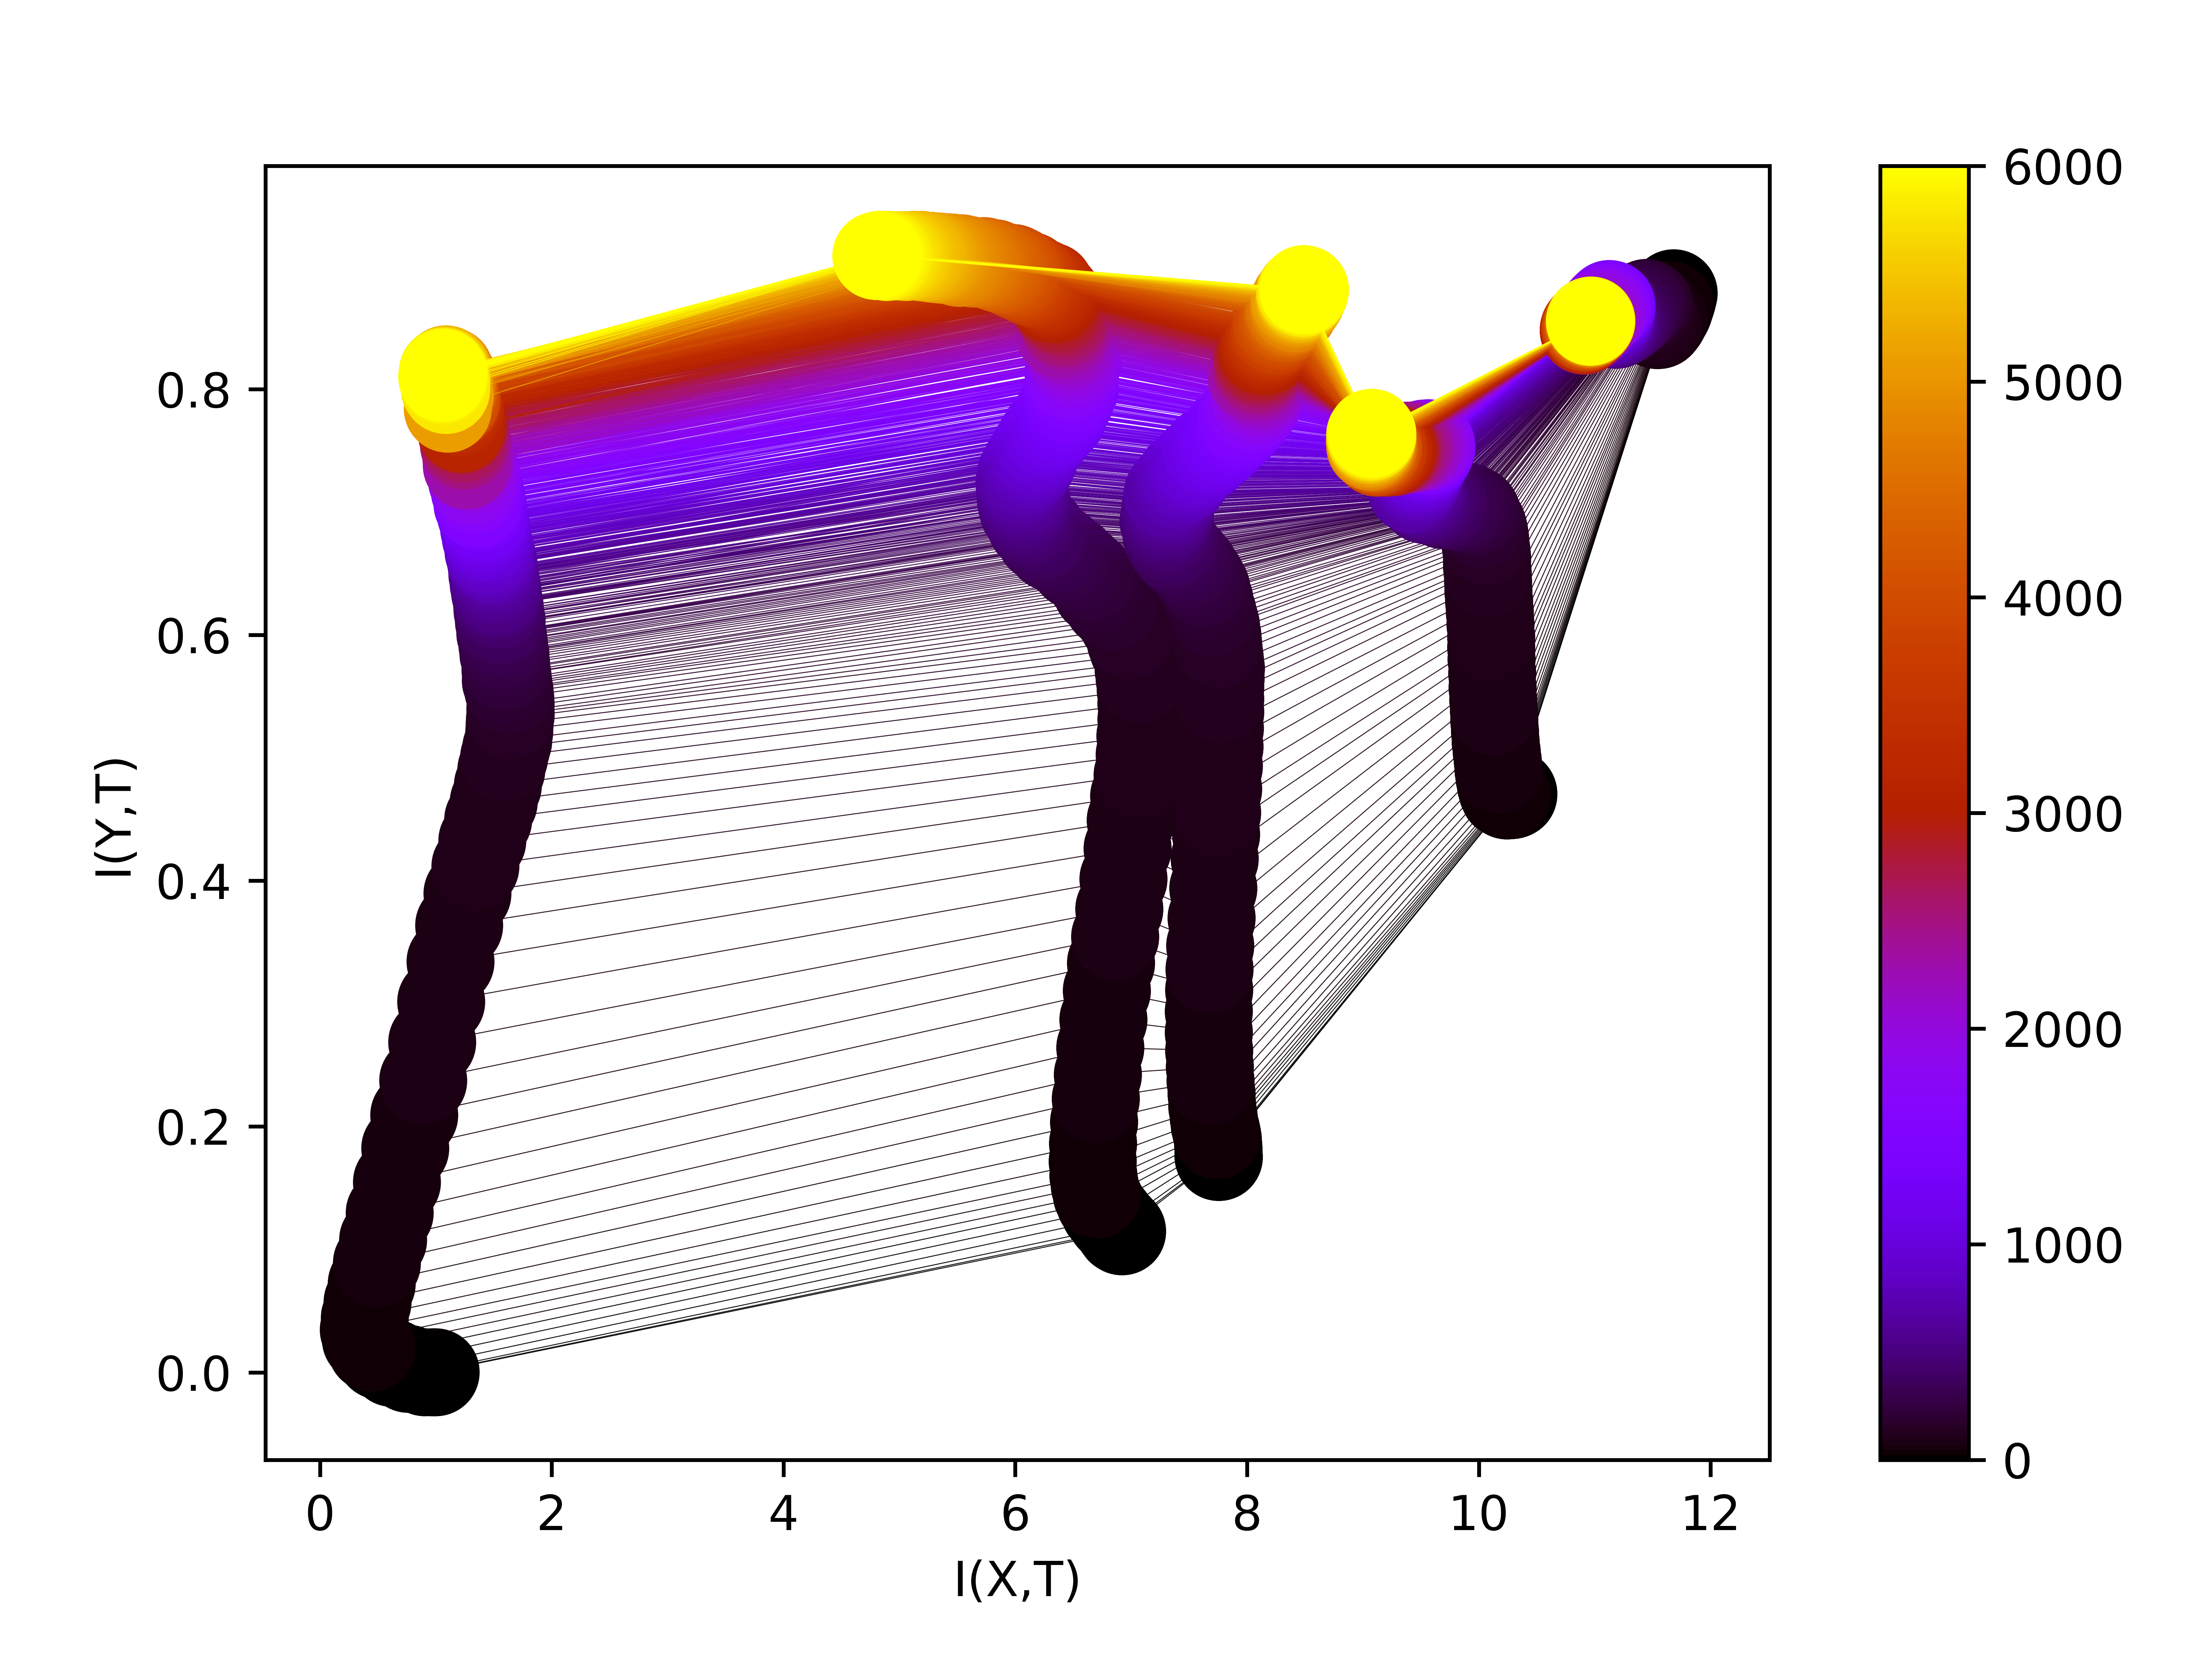
\includegraphics[width=\textwidth]{figs/eval/networkShape/KDE12,12,12.png}
    \caption{
      Network Shape - 12,12,12,12,2
    }
    \label{figNetworkShape3}
  \end{subfigure}
  \hfill
  \caption{
      $\tanh$: Demonstrating KDE for different network shapes.  Tweaking training
      size for Tishby's KDE MIE. Hyperparameters: Dataset - Tishby's, activation
      function - $\tanh$, batch size - 512, training size - 40\%.
    }
  \label{figNetworkShapes}
\end{figure}

% KDE Training Set
\begin{figure}[ht]
  \centering
  \begin{subfigure}[t]{0.32\textwidth}
    \centering
    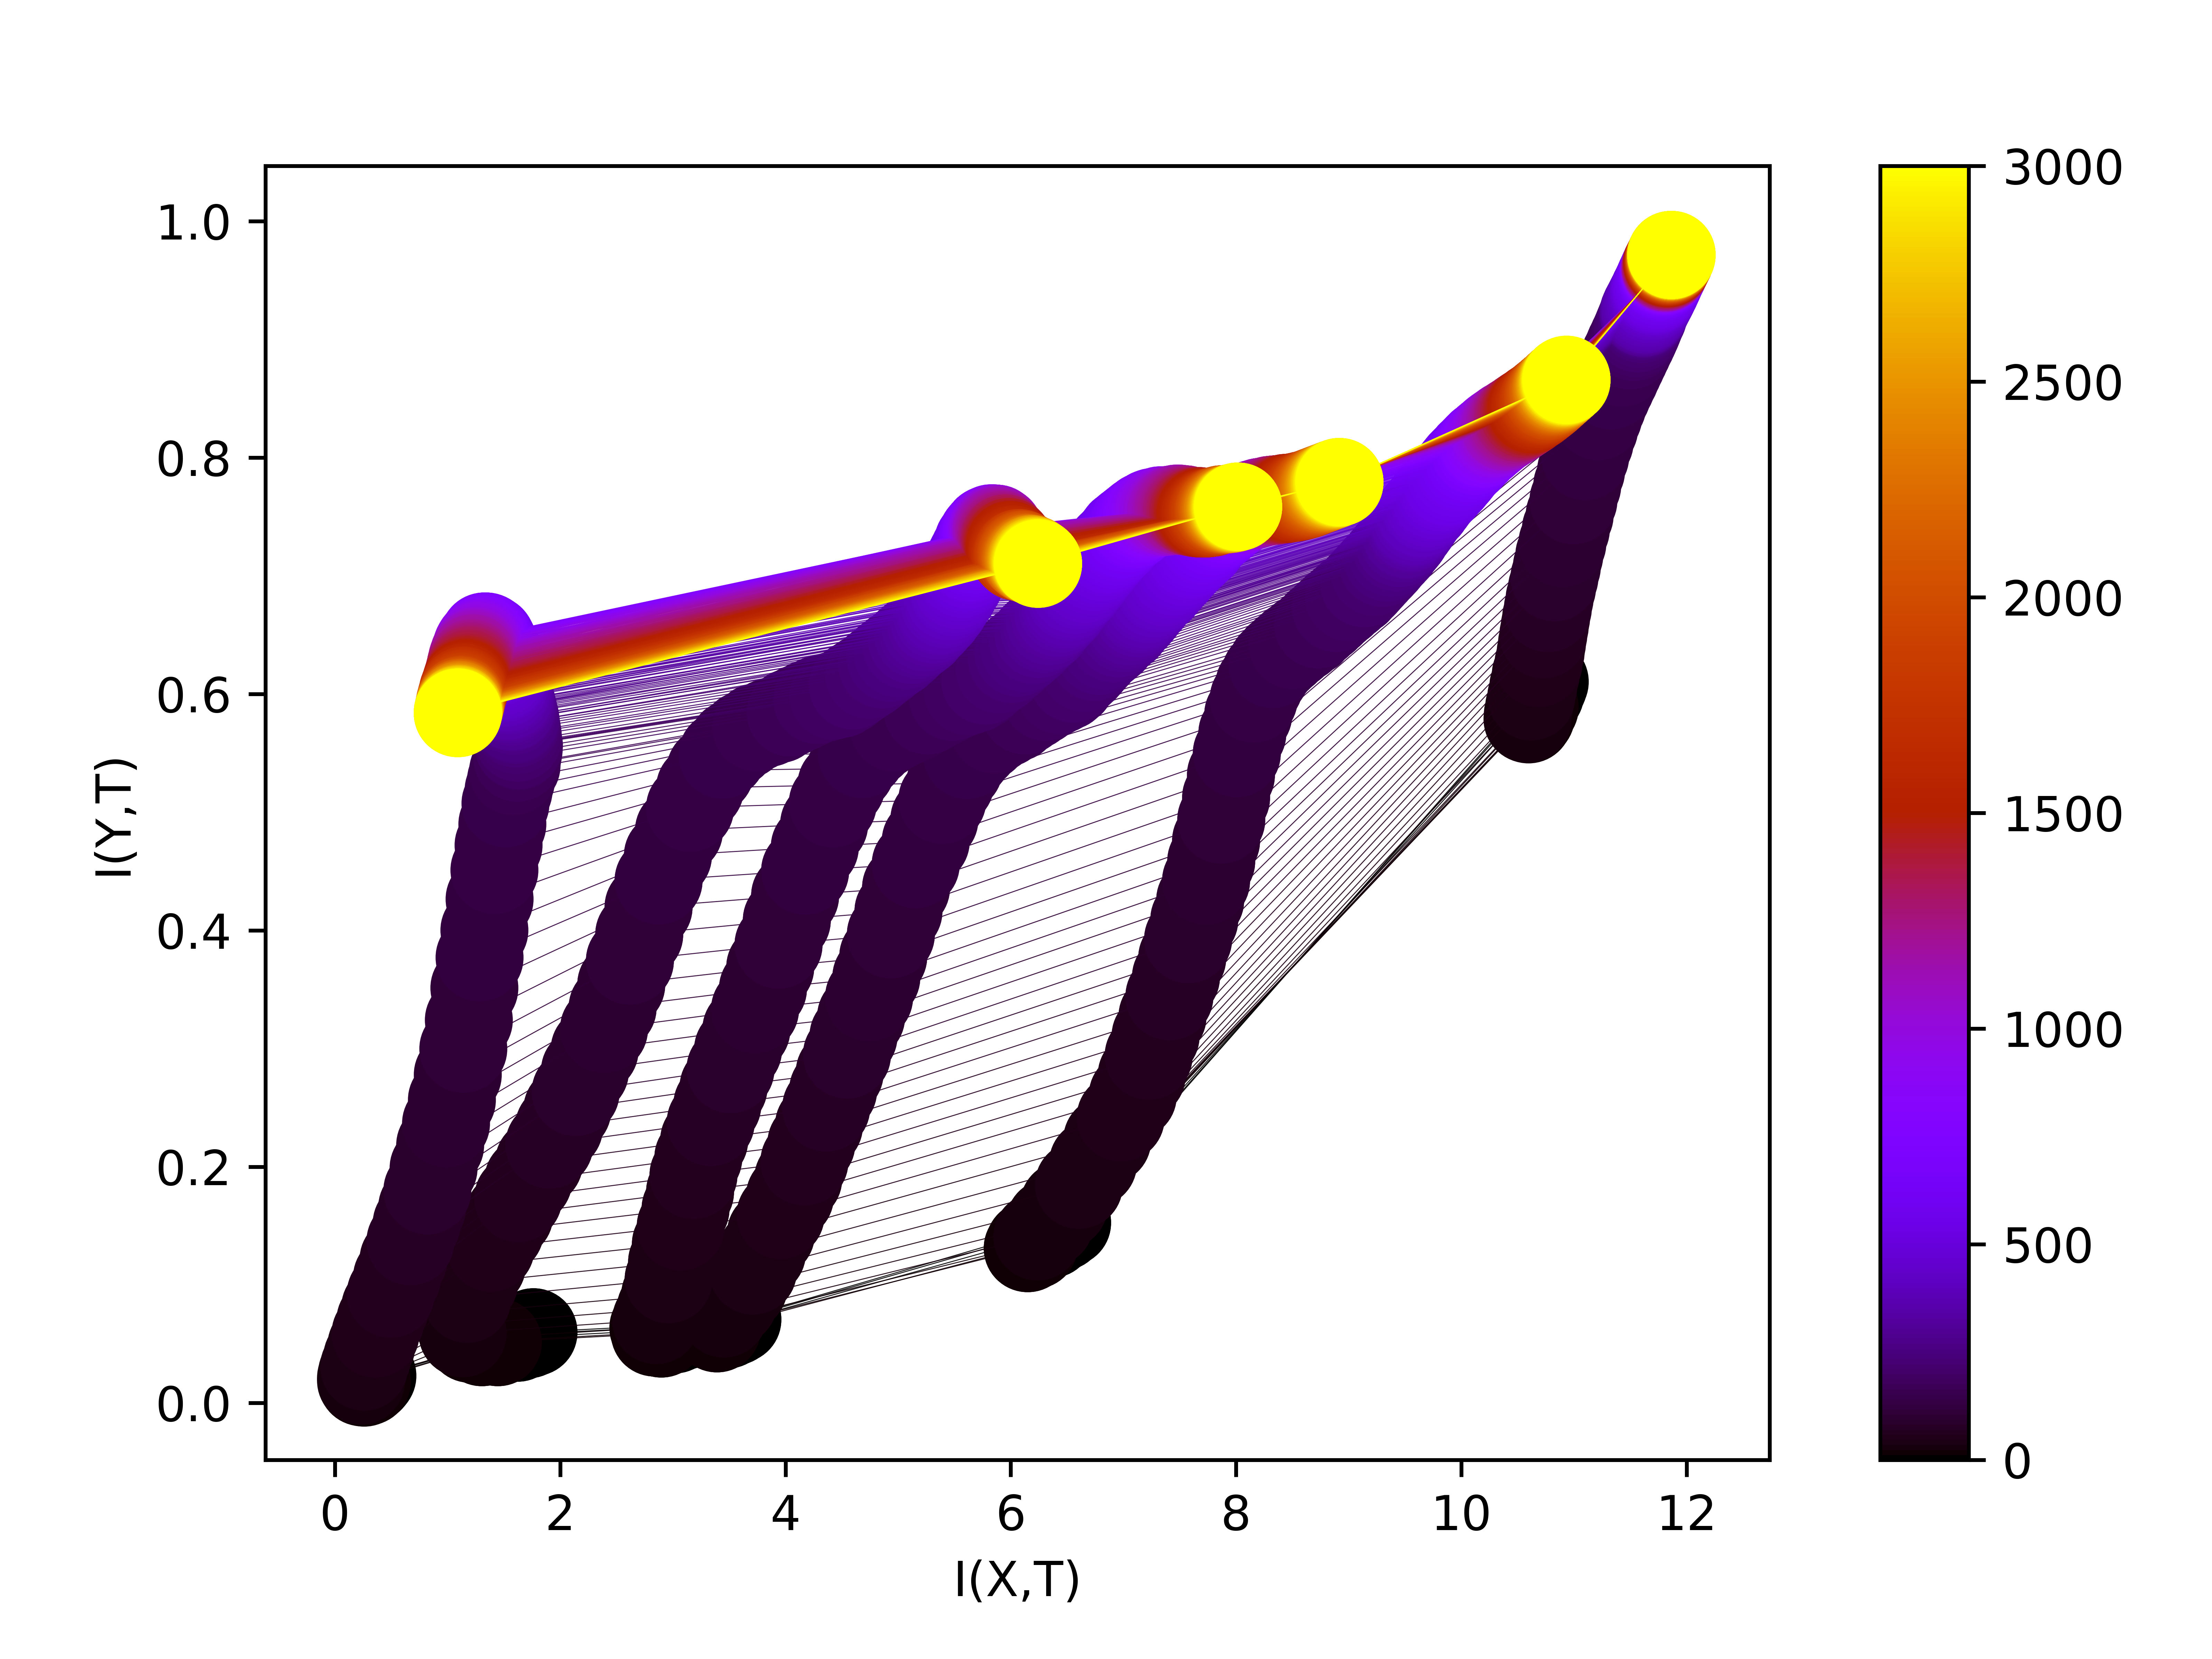
\includegraphics[width=\textwidth]{figs/eval/trainingSizeRelu/KDE20.png}
    \caption{
      Training size - 20\%
    }
  \end{subfigure}
  \begin{subfigure}[t]{0.32\textwidth}
    \centering
    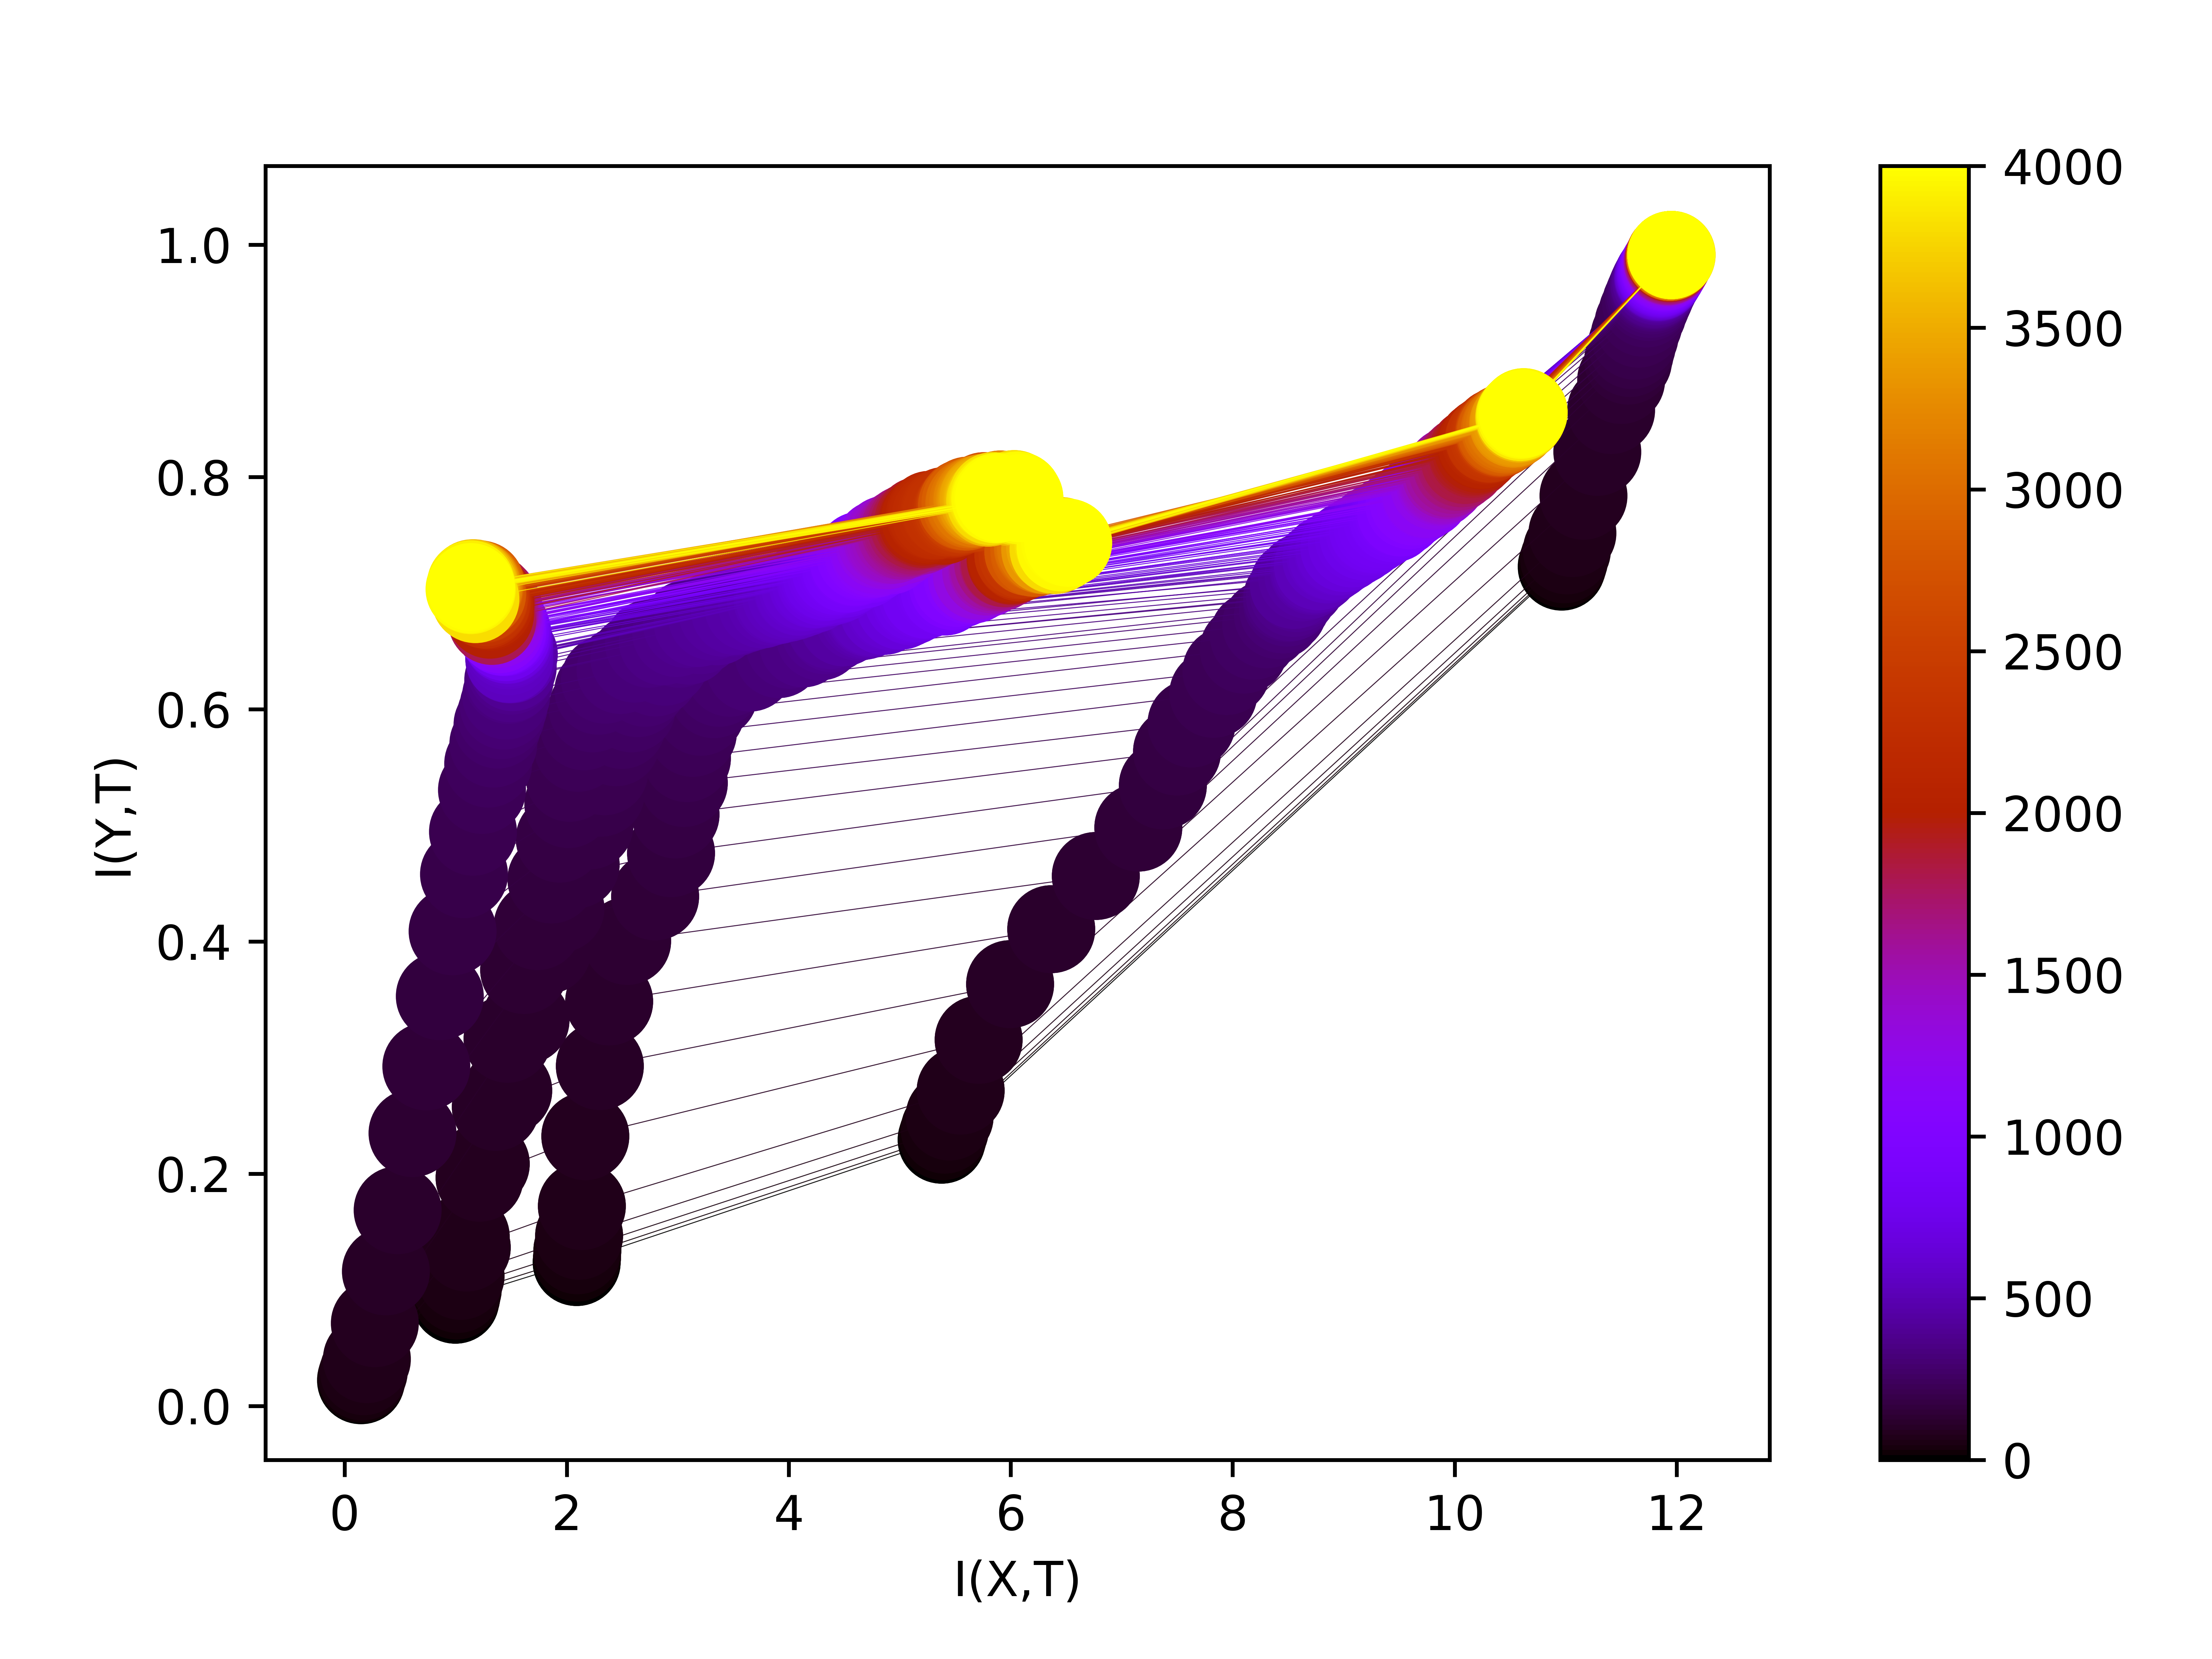
\includegraphics[width=\textwidth]{figs/eval/trainingSizeRelu/KDE40.png}
    \caption{
      Training size - 40\%
    }
  \end{subfigure}
  \begin{subfigure}[t]{0.32\textwidth}
    \centering
    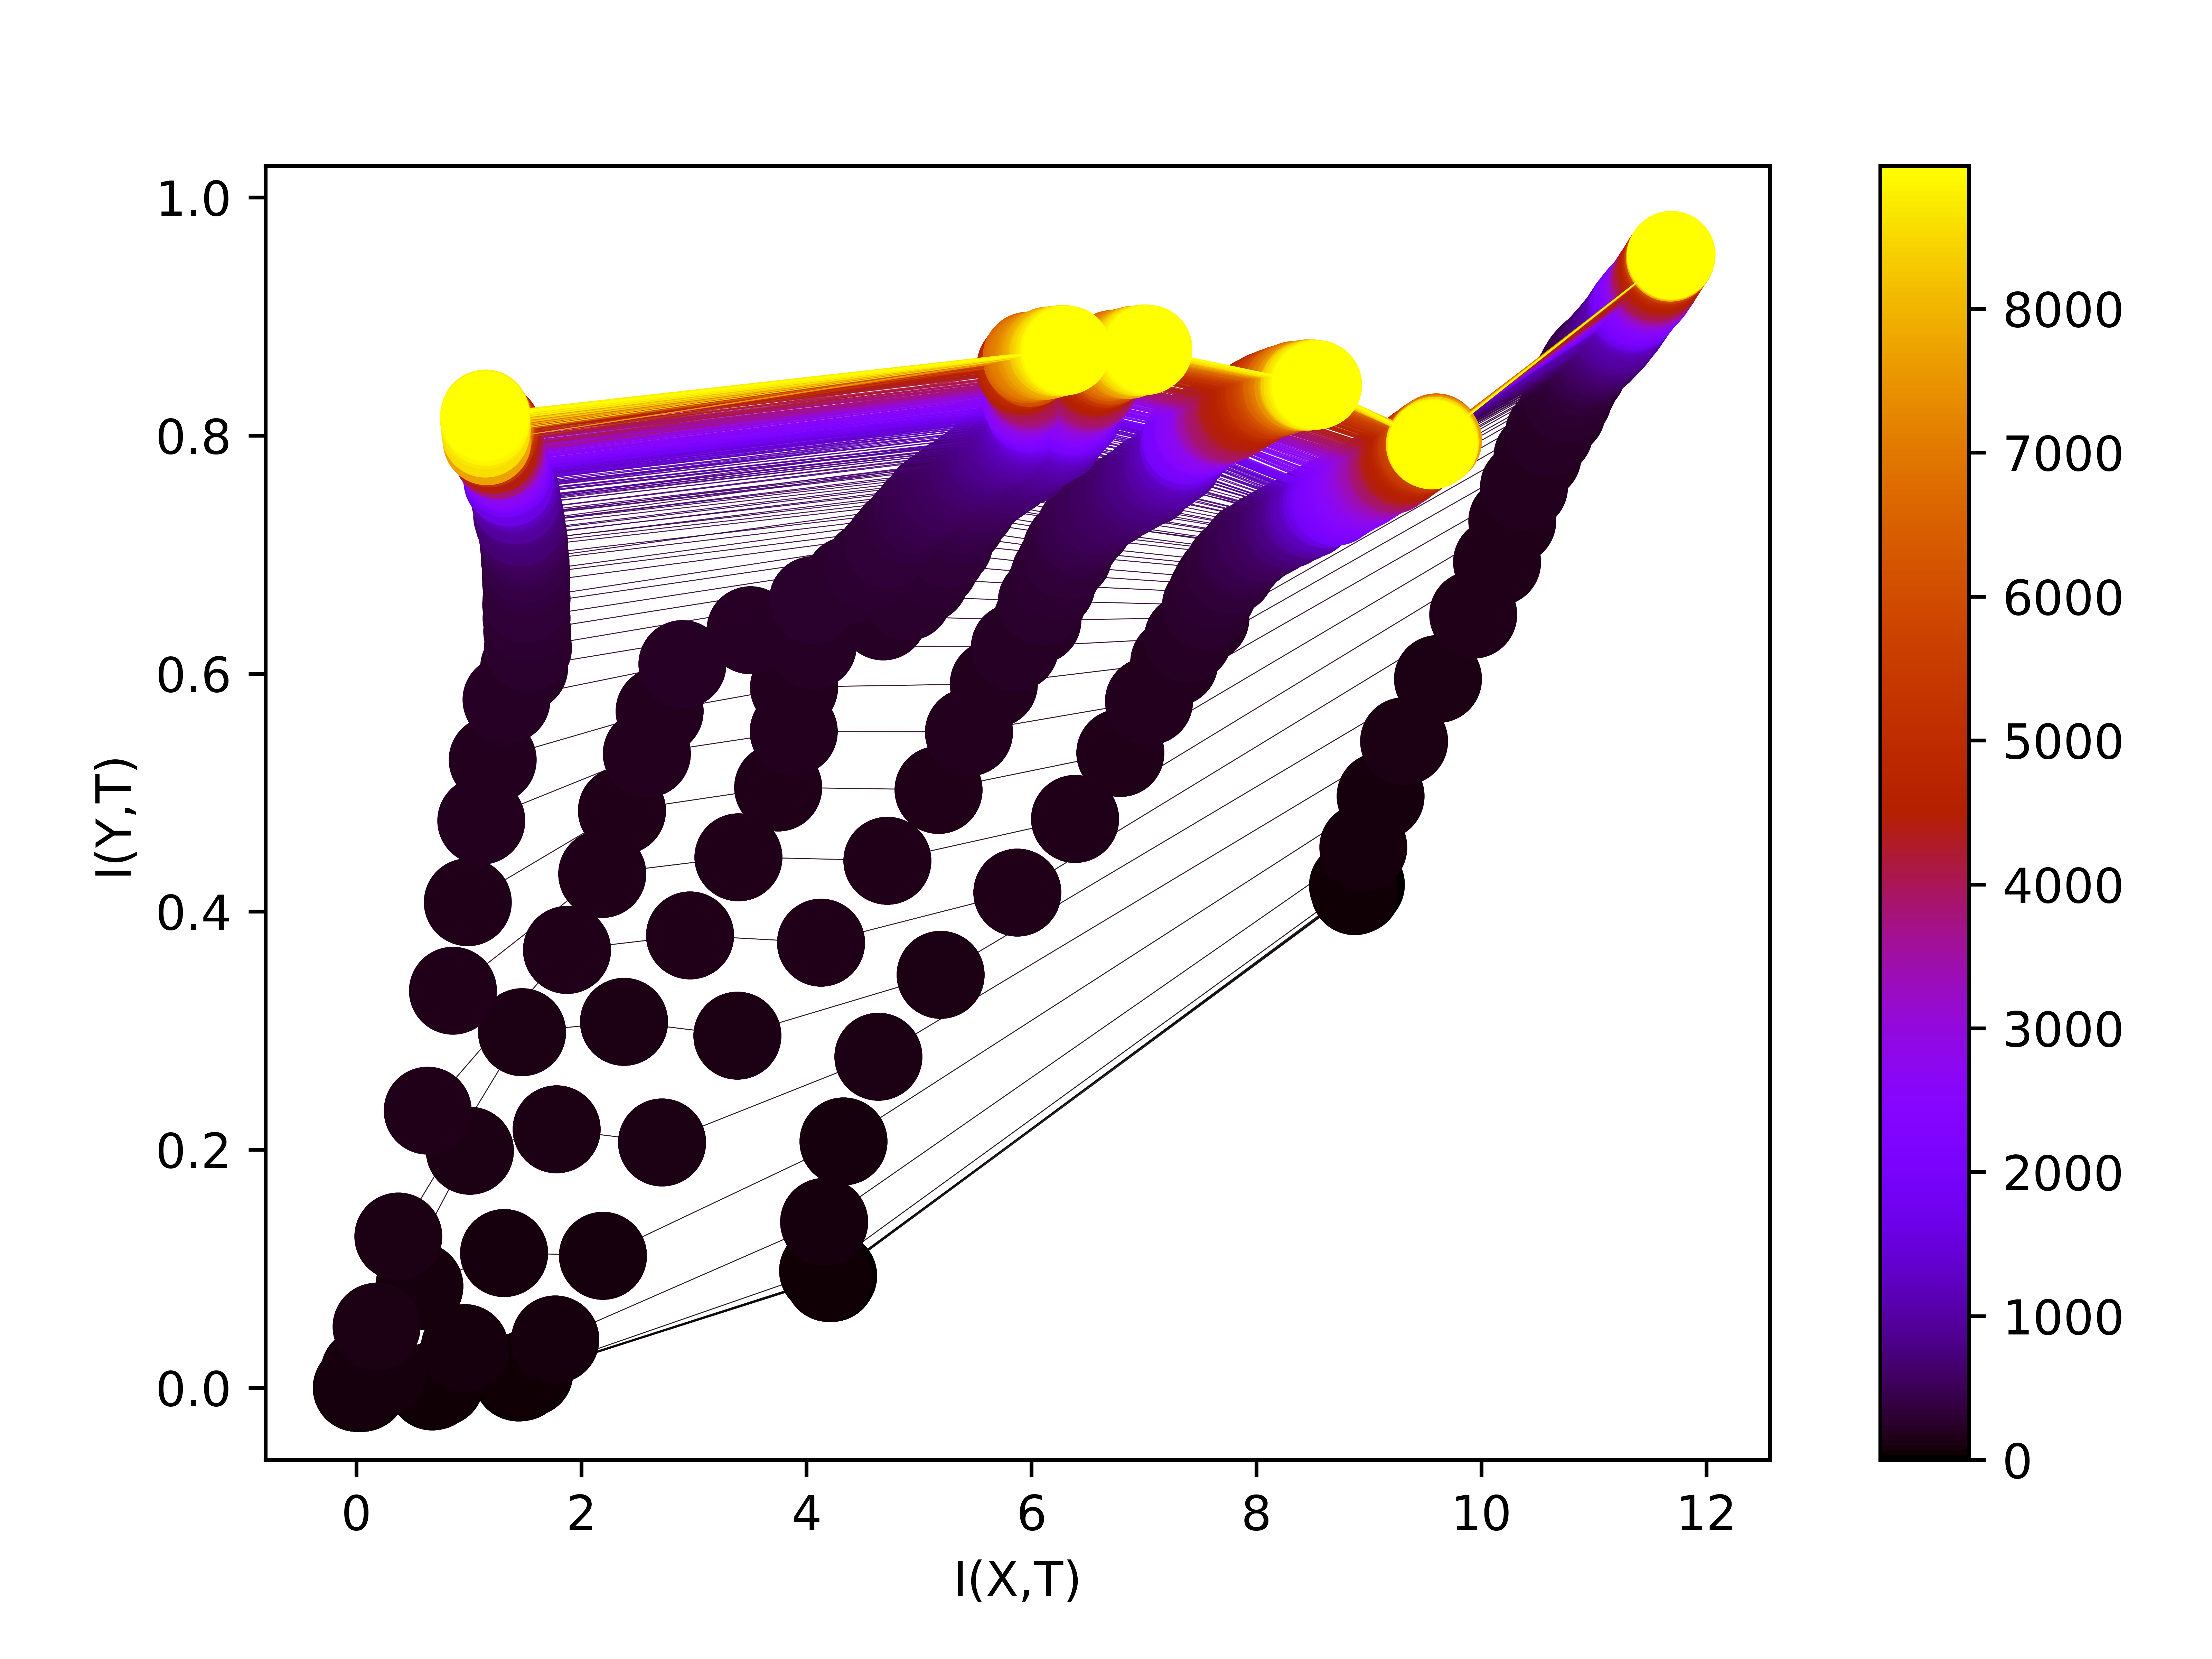
\includegraphics[width=\textwidth]{figs/eval/trainingSizeRelu/KDE70.png}
    \caption{
      Training size - 70\%
    }
  \end{subfigure}
  \caption{
      ReLu: Demonstrating KDE for different training sizes.  Tweaking training
      size for Tishby's KDE MIE. Hyperparameters: Dataset - Tishby's, activation
      function - $\tanh$, batch size - 512, network shape 12,10,8,6,4,2.
    }
  \label{figKDETSRelu}
\end{figure}
  
\begin{figure}[ht]
  \centering
  \begin{subfigure}[t]{0.32\textwidth}
    \centering
    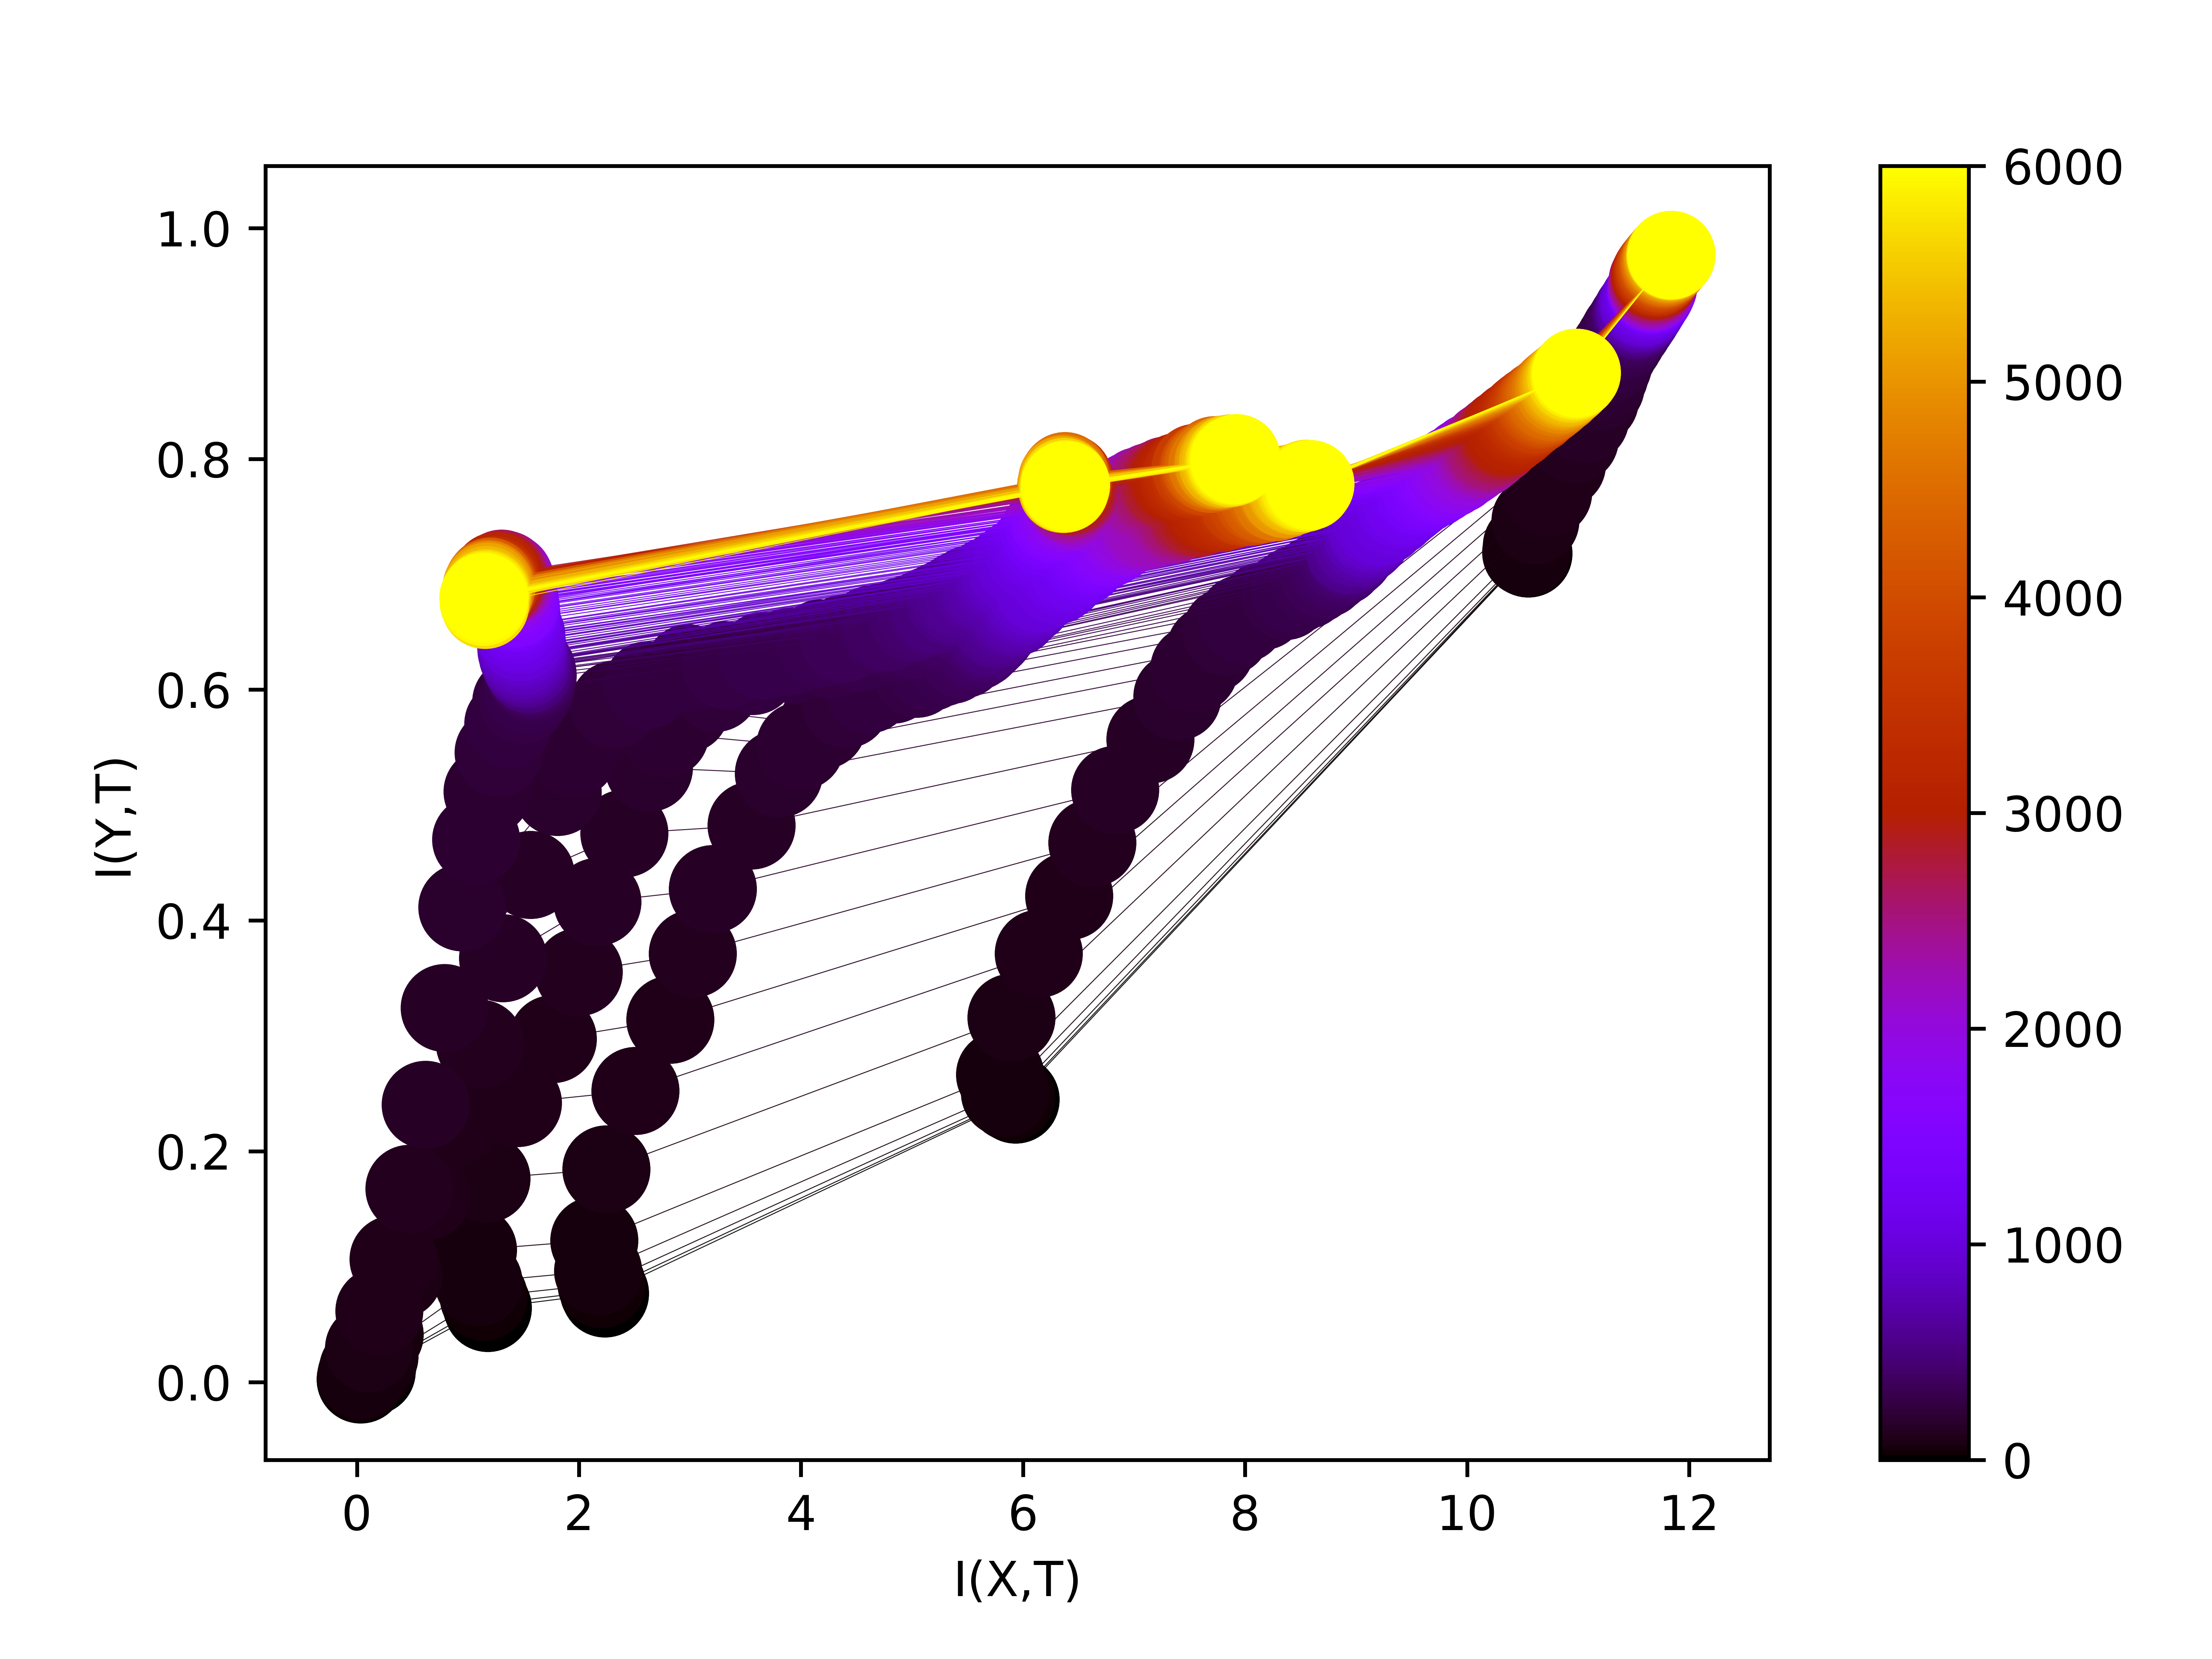
\includegraphics[width=\textwidth]{figs/eval/networkShapeRelu/KDE1.png}
    \caption{
      Network Shape - 12,10,8,6,4,2, Default
    }
  \end{subfigure}
  \hfill
  \begin{subfigure}[t]{0.32\textwidth}
    \centering
    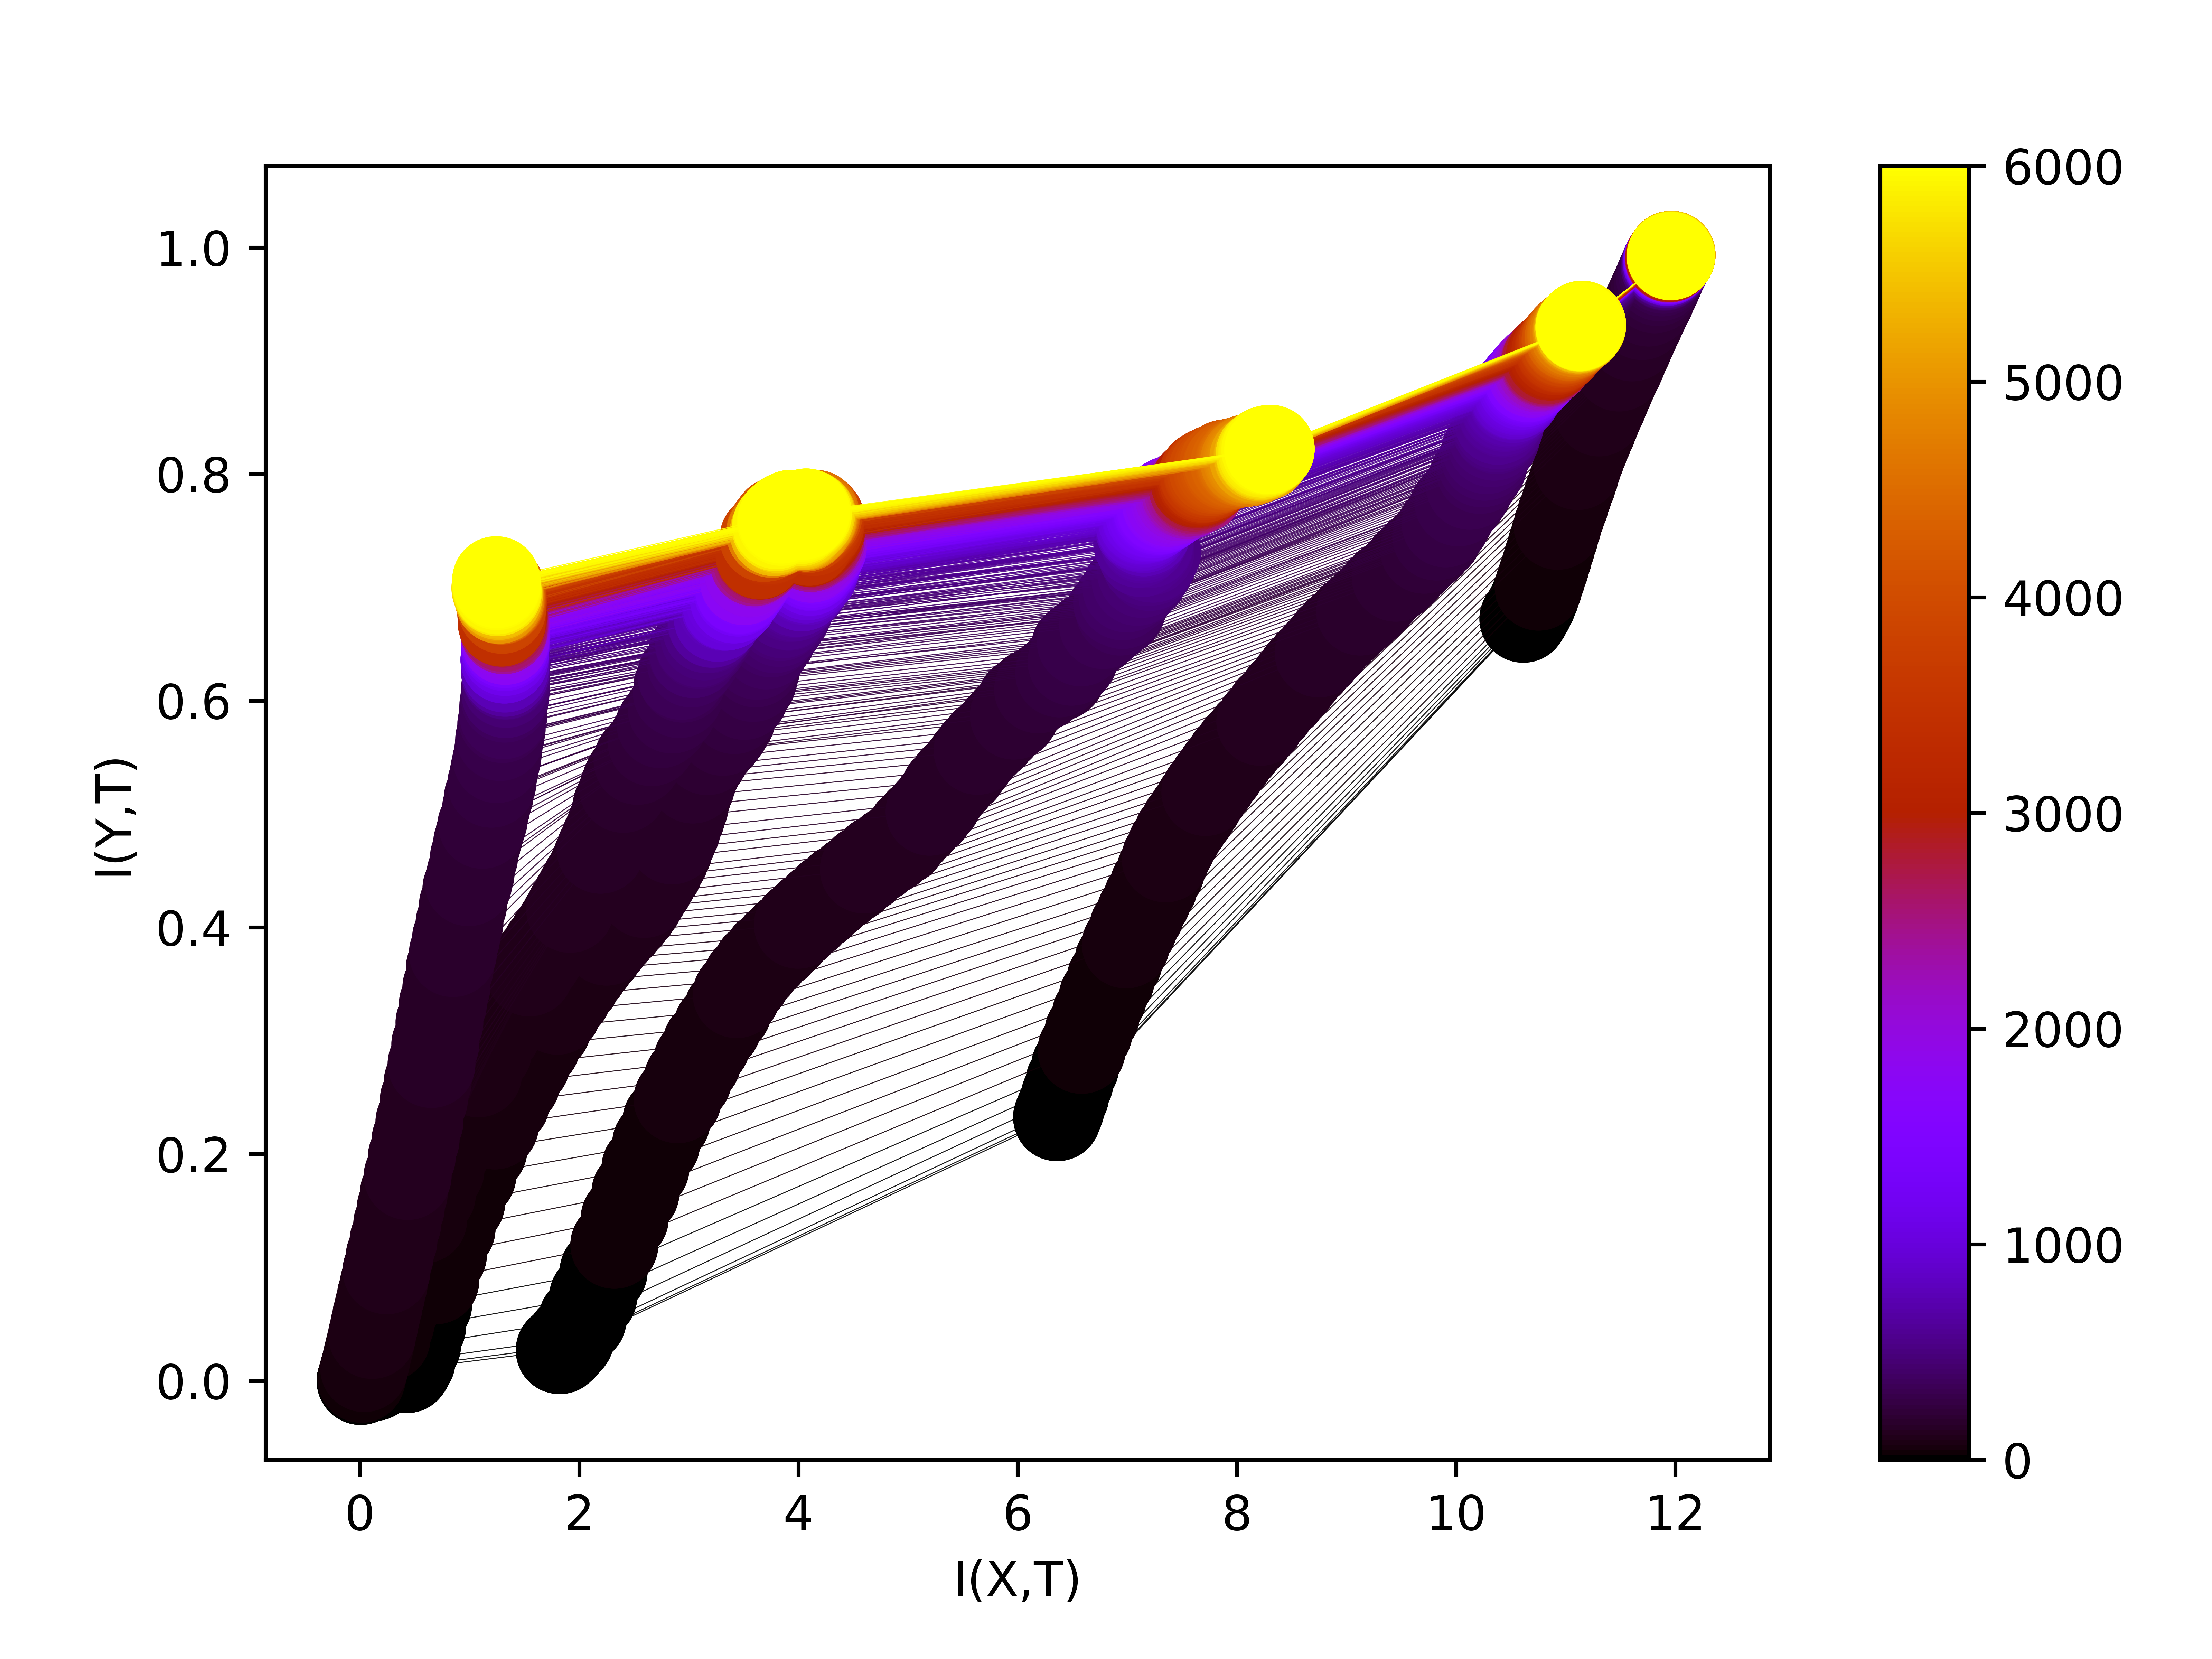
\includegraphics[width=\textwidth]{figs/eval/networkShapeRelu/KDE2.png}
    \caption{
      Network Shape - 12,10,4,2,2,2
    }
  \end{subfigure}
  \hfill
  \begin{subfigure}[t]{0.32\textwidth}
    \centering
    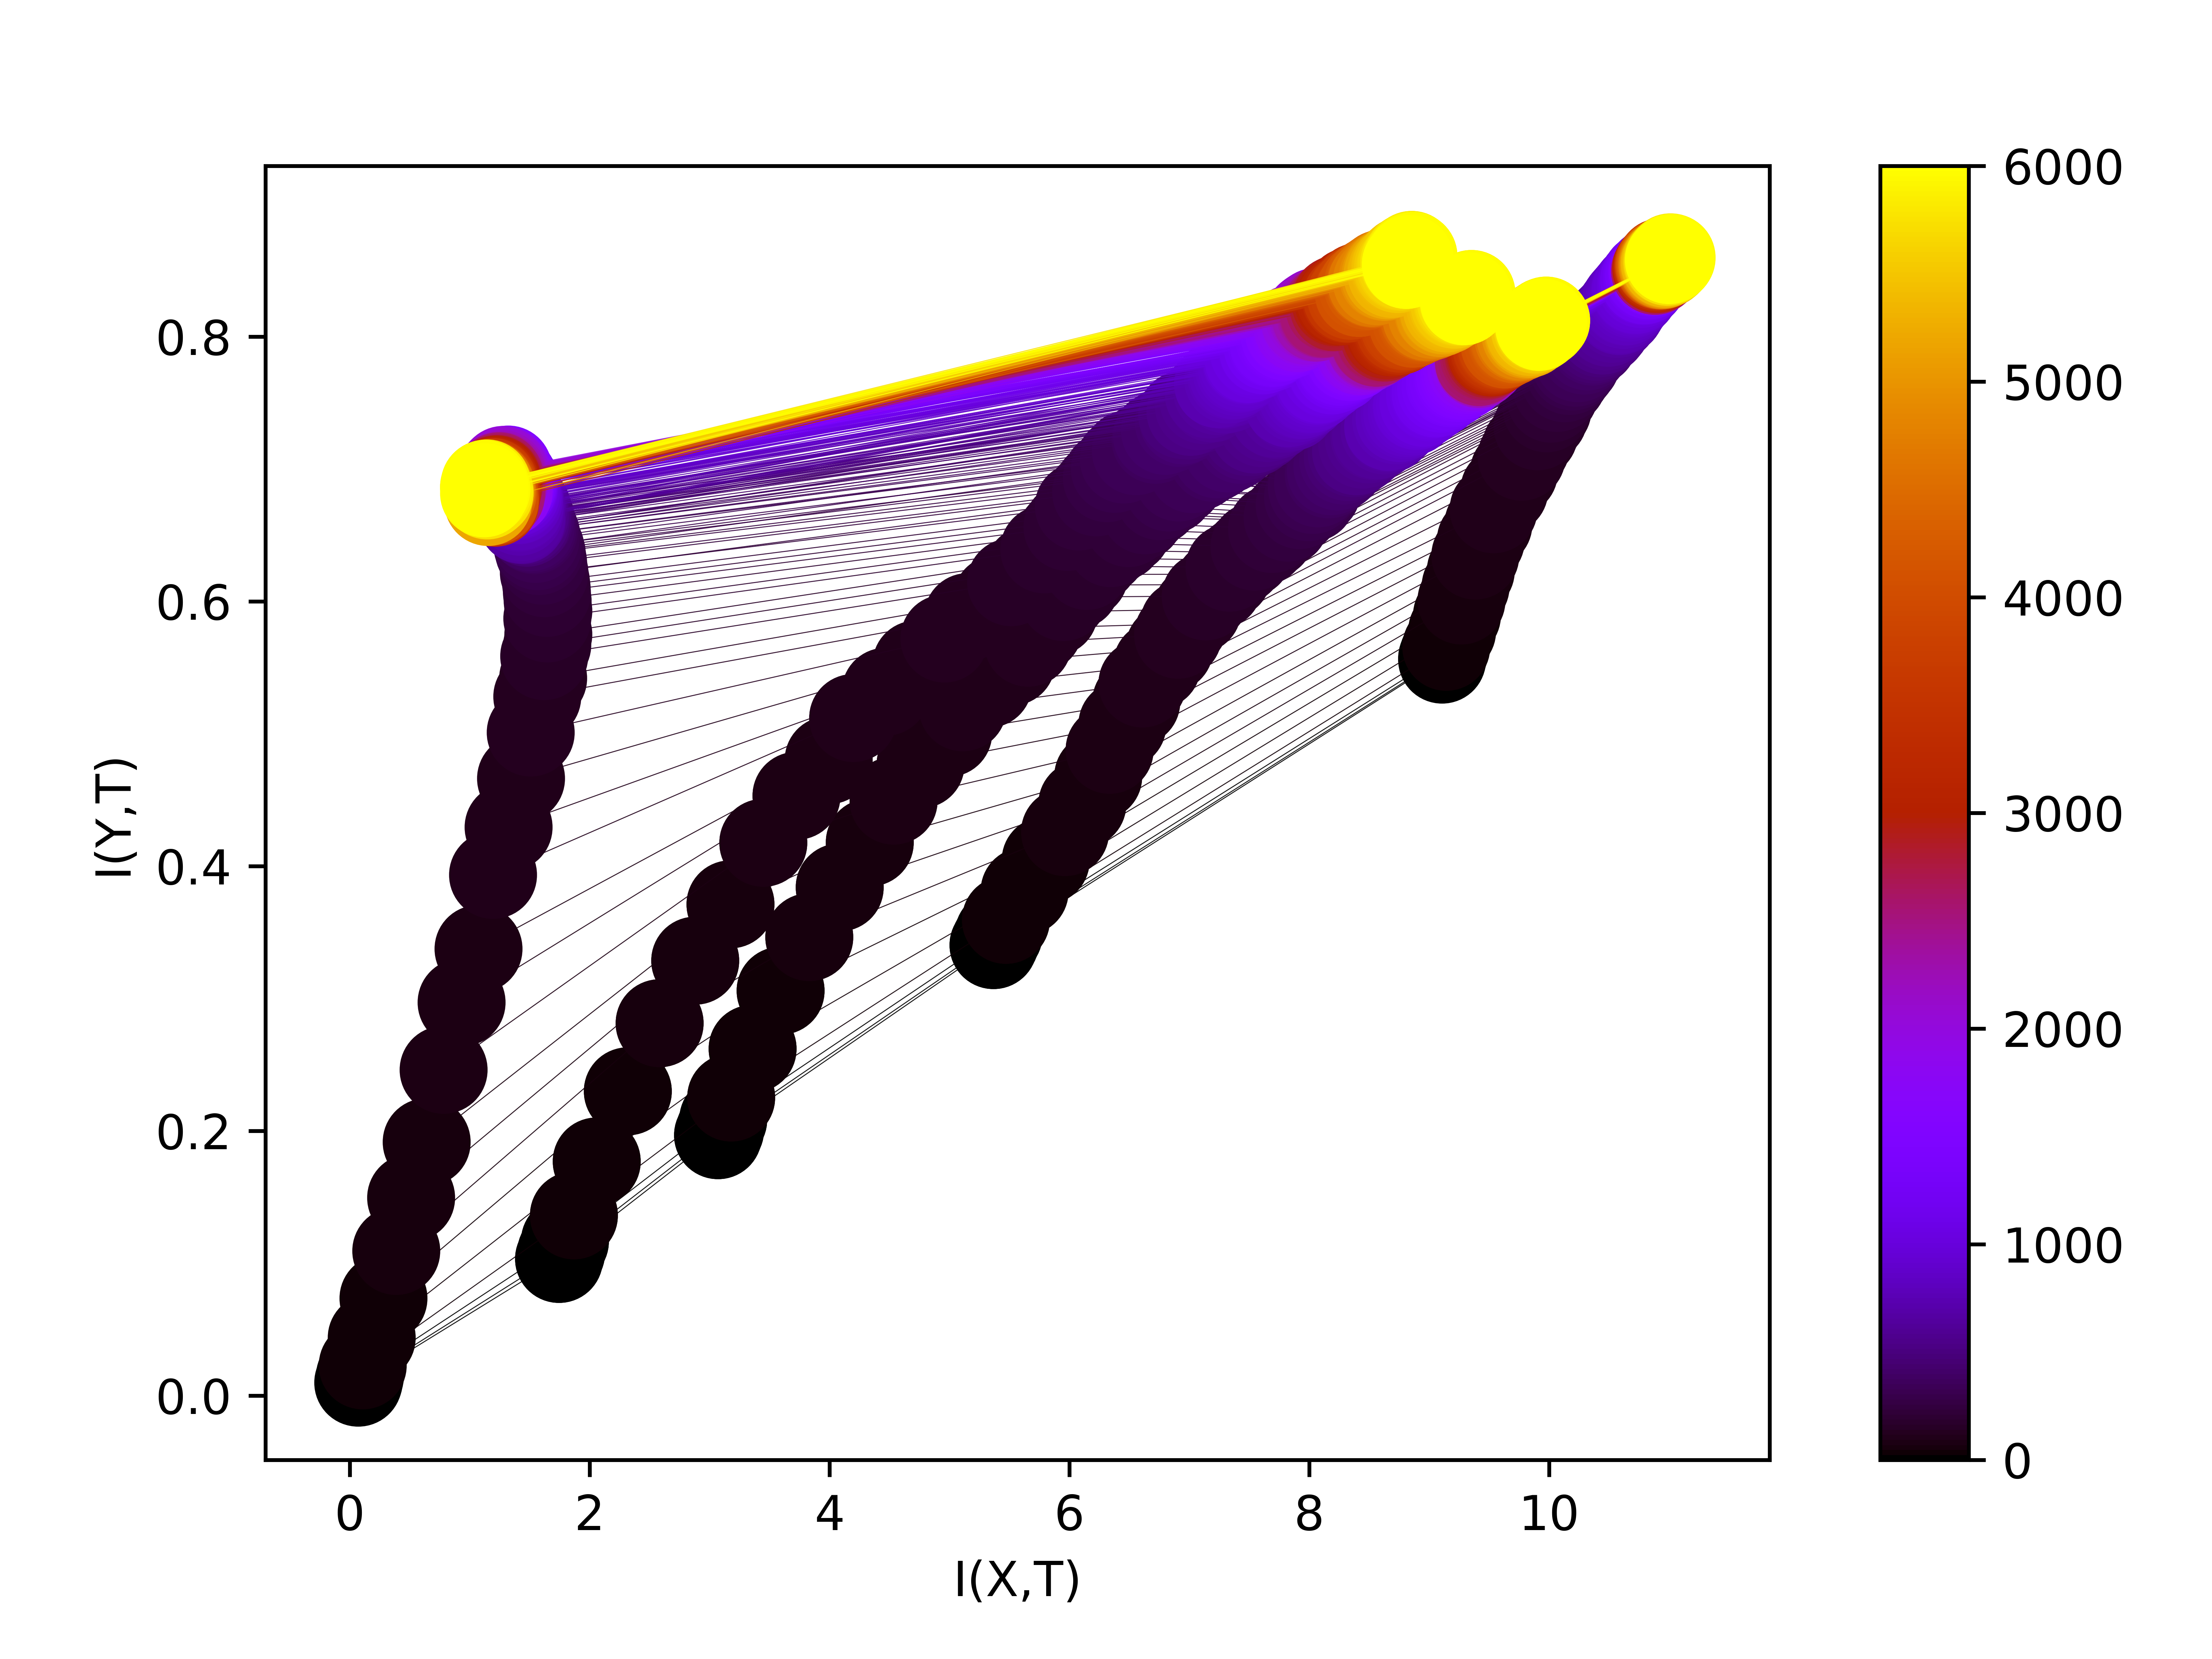
\includegraphics[width=\textwidth]{figs/eval/networkShapeRelu/KDE3.png}
    \caption{
      Network Shape - 12,12,12,12,2
    }
  \end{subfigure}
  \hfill
  \caption{
      ReLu: Demonstrating KDE for different network shapes.  Tweaking training
      size for Tishby's KDE MIE. Hyperparameters: Dataset - Tishby's, activation
      function - ReLu, batch size - 512, training size - 40\%.
    }
  \label{figNetworkShapesReLu}
\end{figure}

\end{document}
